\clearpage
\section{Appendix}
\label{app:A}

\subsection{Data Description}
\label{app:A1}

\begin{table}[H]
\centering
\begin{tabular}{p{0.2\textwidth}p{0.75\textwidth}}
\toprule
Data inputs & Description \\
\midrule
start\_time
& 
Time where trips are started : datetime  \\

end\_time
&
Time where trips are finished : datetime \\

start\_station\_id
&
ID for start station : integer   \\

start\_station\_name 
&
Name for start station : string \\

end\_station\_name 
&
Name for end station : string \\

bike\_id 
&
ID for unique bike : integer \\

user\_type 
&
Subscriber and customer are distinguished : string \\

duration\_time 
&
Duration of trip (in sec., min., hour) : integer \\

weekday\_start 
&
Indicating weekday (true/false) : boolean \\

full\_hour\_start 
&
Start time rounded to full hour : datetime \\

max\_temp 
&
Describing temperature values in Celsius : float \\

precip 
&
Indicating rain/snow (true/false) : boolean \\

total\_docks 
&
Theoretical maximum capacity of the station : integer \\

docks\_in\_service 
&
Actual capacity of the station : integer \\

status 
&
Availability of the stations : string \\

start\_latitude 
&
Latitude of the starting station : float \\

start\_longitude 
&
Longitude of the start station : float \\






\bottomrule
\end{tabular}
\caption[Data description of most relevant data inputs]{Data description of most relevant data inputs}
\label{tab:dataDescription}
\end{table} \\


\subsection{Temporal Demand Patterns and Seasonality}
\label{app:A2}

\begin{figure}[H]
    \centering
    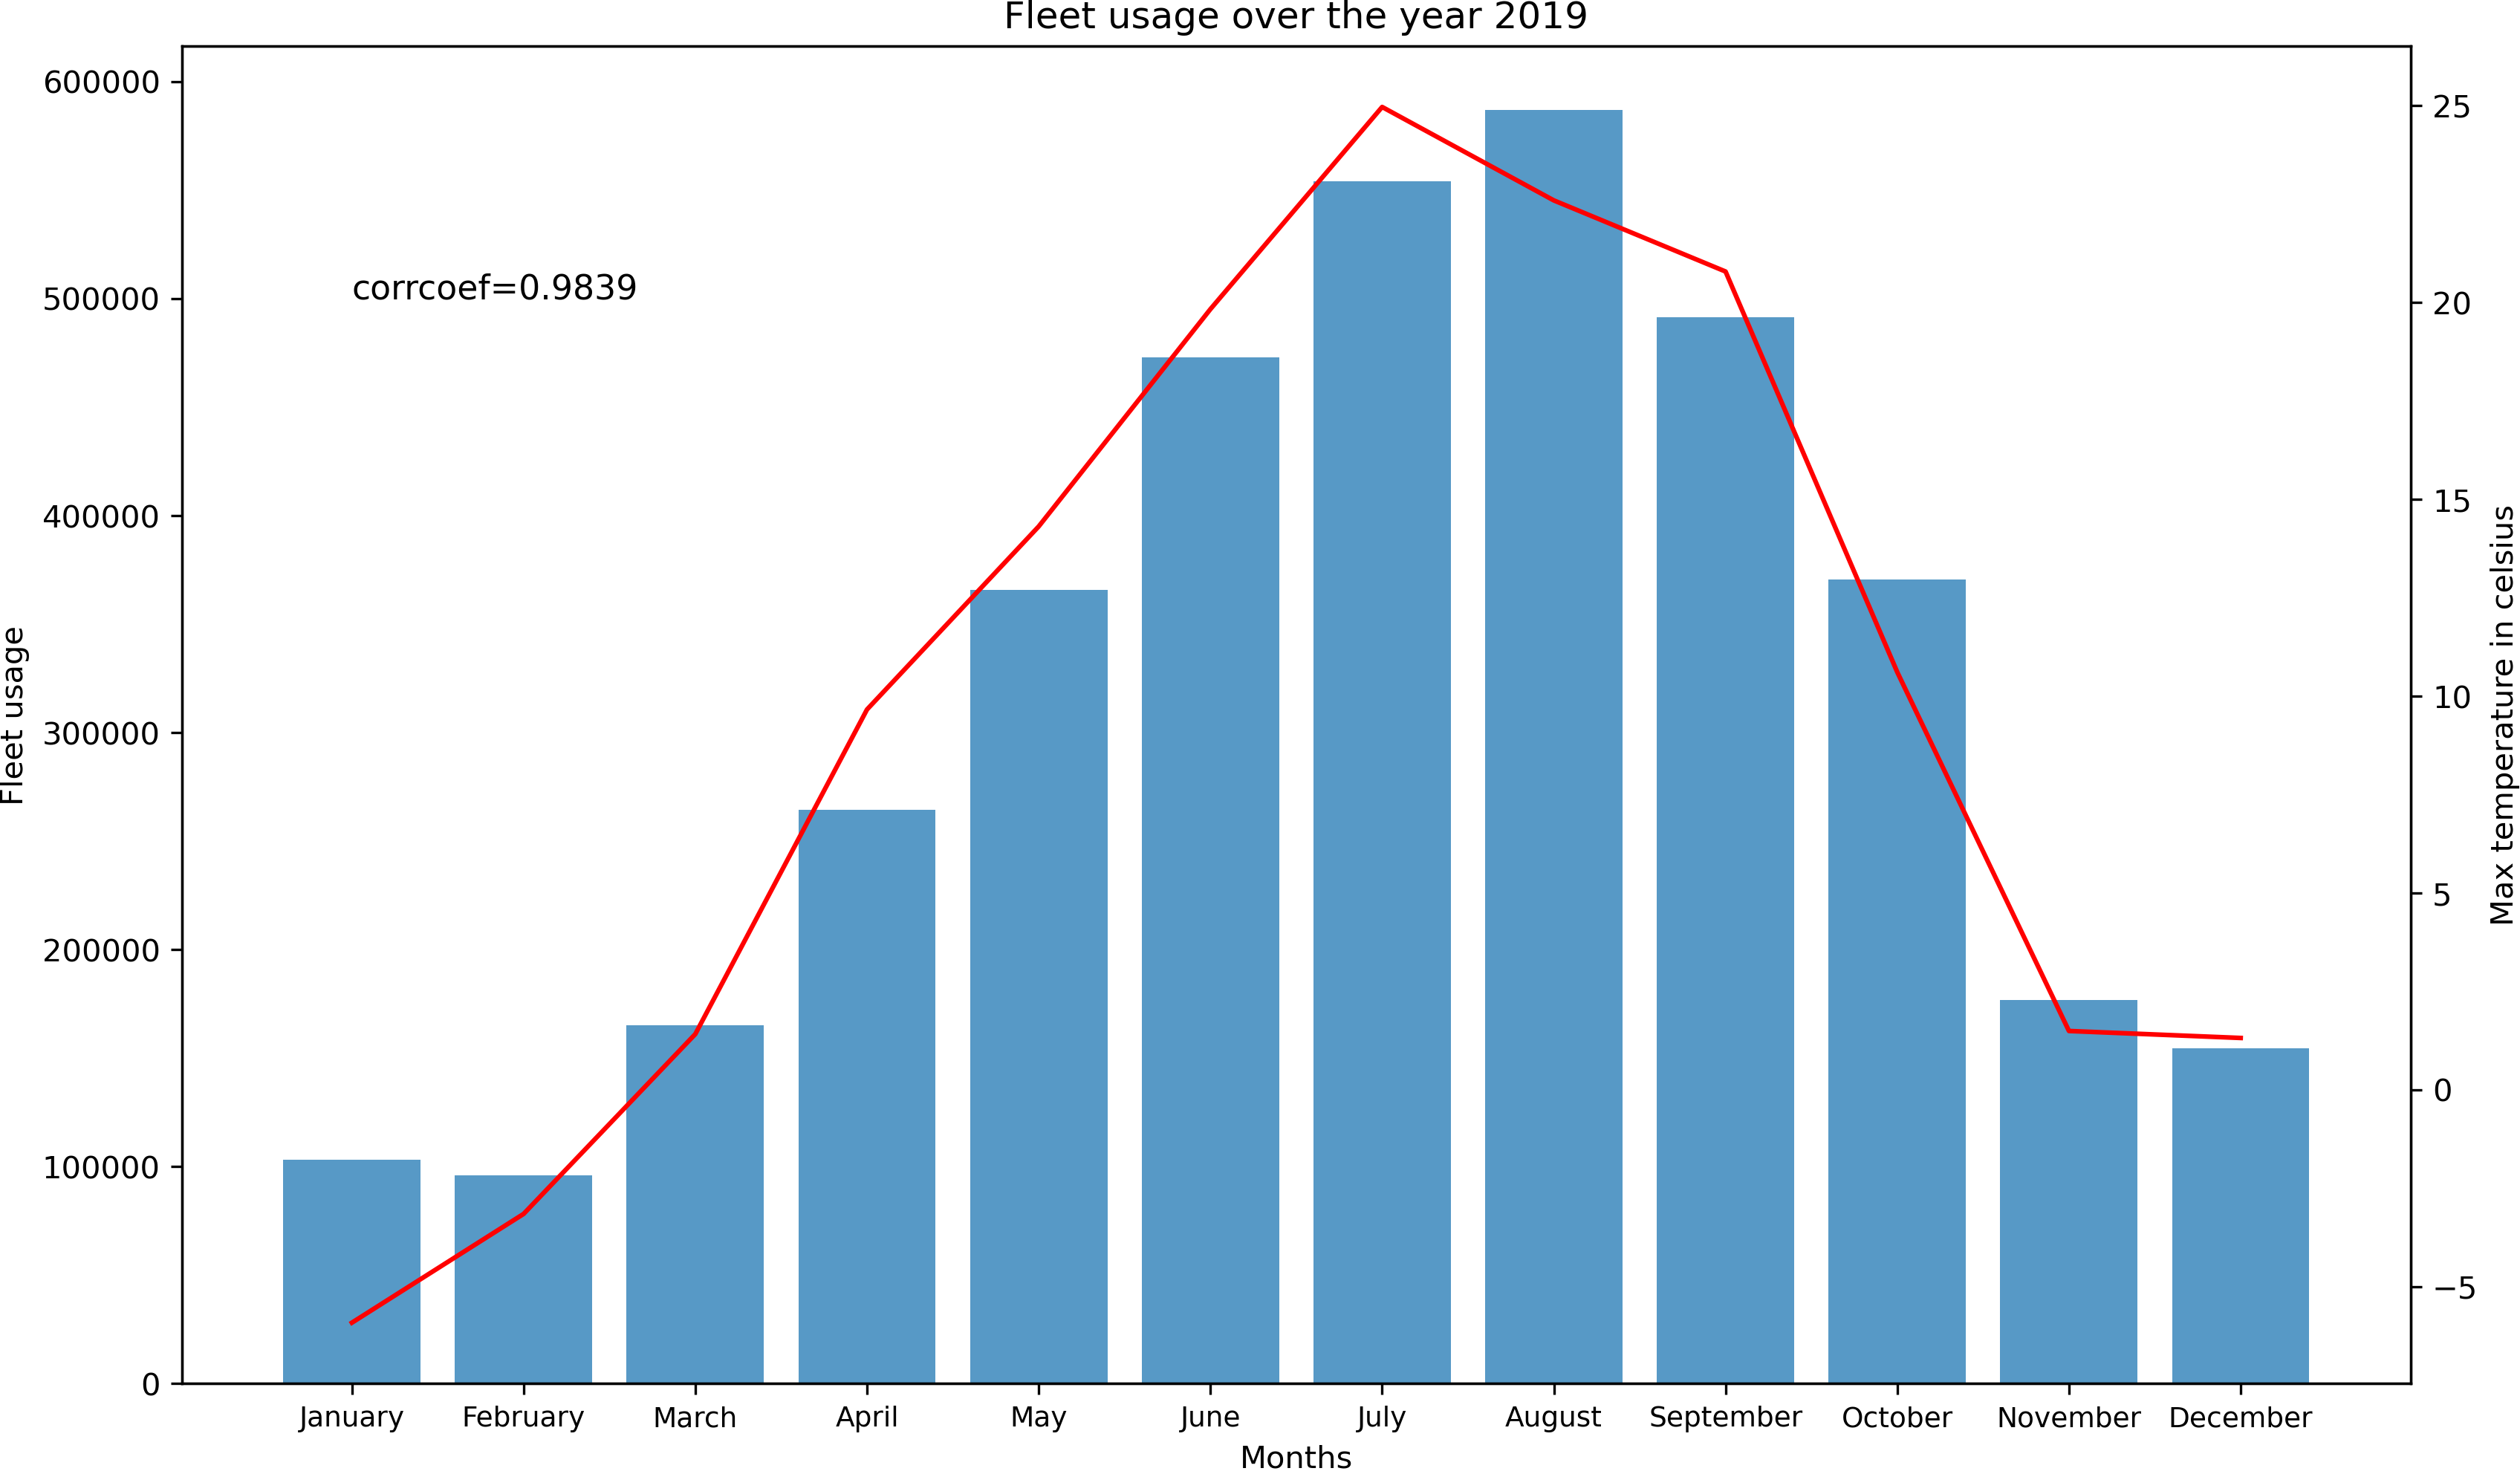
\includegraphics[width=1\linewidth]{./Figures/fleetUsageYear.png}
    \caption{Fleet usage over the year 2019}
    \label{fleetUsageYear}
\end{figure}

\begin{figure}[H]
    \centering
    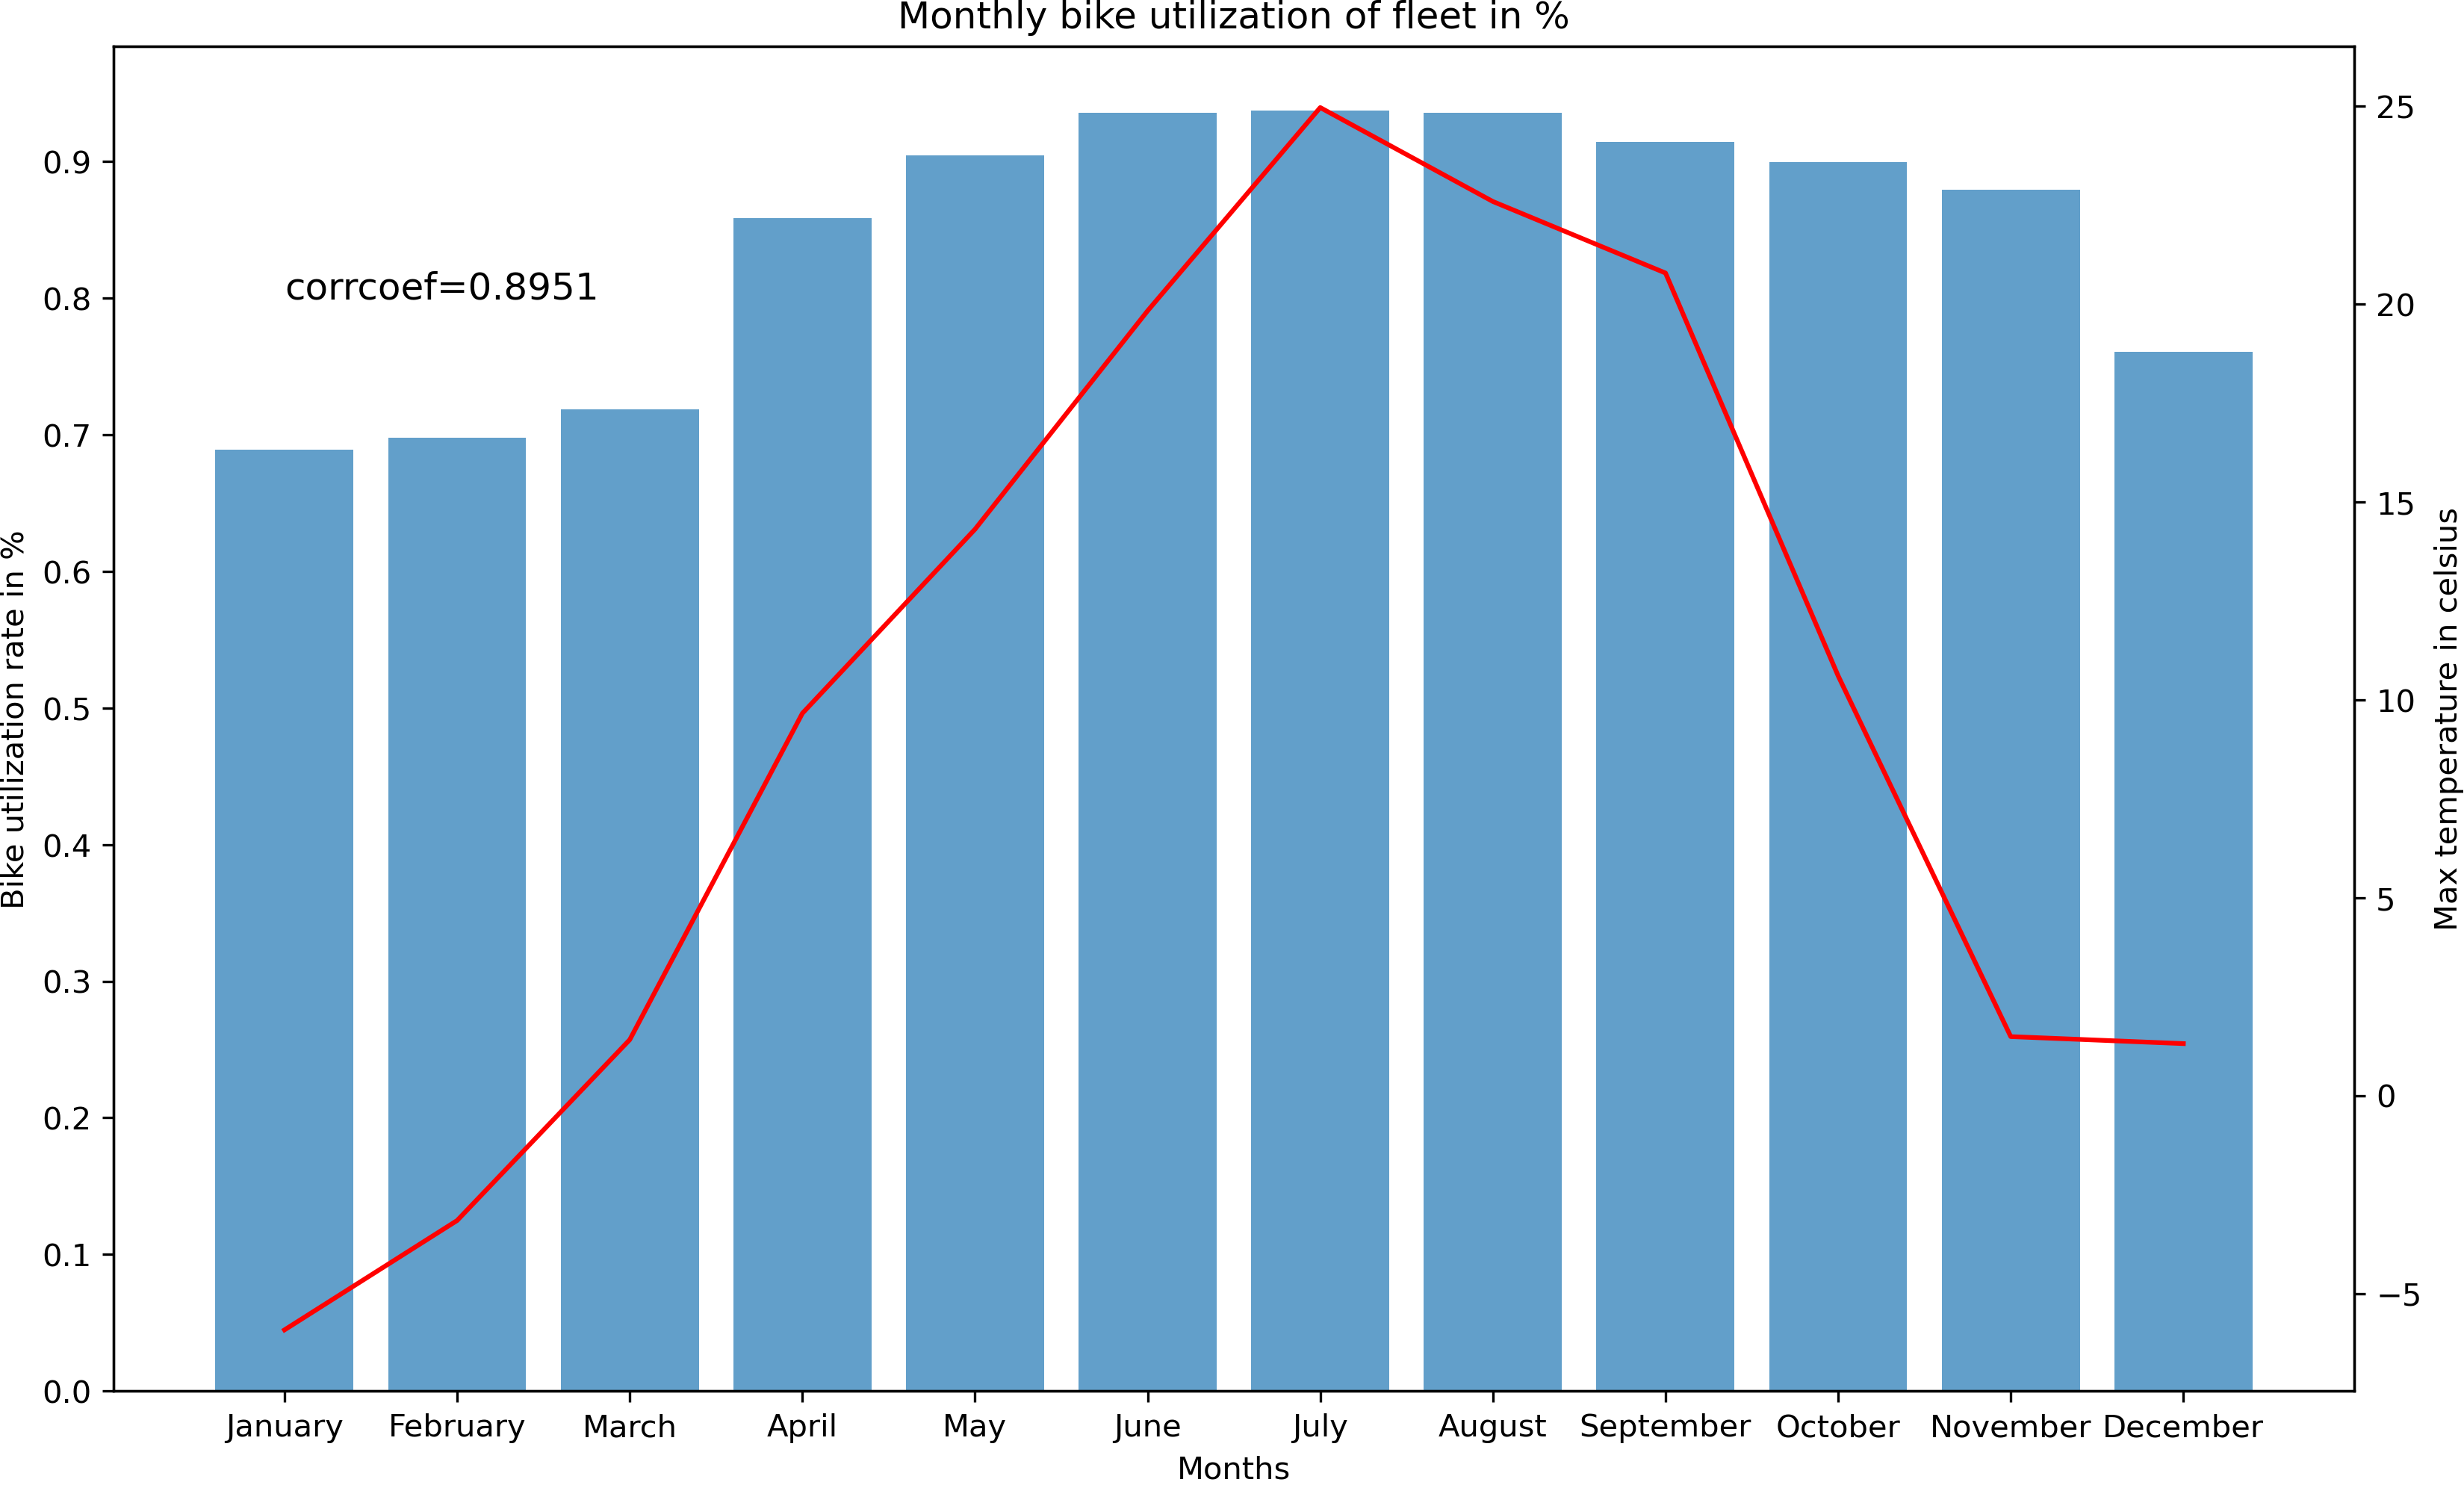
\includegraphics[width=1\linewidth]{./Figures/fleetUtilizationYear.png}
    \caption{Bike utilization over the year 2019}
    \label{fleetUtilizationYear}
\end{figure}

\begin{figure}[H]
   \centering
    \includegraphics[width=0.8\linewidth]{./Figures/DailyUsageWithPrecip.png}
    \caption{Daily bike usage of fleet with precip for each month}
    \label{DailyUsageWithPrecip}
\end{figure}

\begin{figure}[H]
   \centering
    \includegraphics[width=0.8\linewidth]{./Figures/DailyUtilizationWithPrecip.png}
    \caption{Daily bike utilization of fleet with precip for each month}
    \label{DailyUtilizationWithPrecip}
\end{figure}

\subsection{KPI 1: RPUB (Rides Per Unique Bike)}
\label{app:A3}

\subsection*{Weather-based investigation of RPUB}
\label{app:A1}

To be able to also take into account some of the weather data, two metrics were developed. Firstly, if more than half of all rides on one day started during rain, then the day was counted as "rainday". Secondly, if the average temperature was above ten degrees, the day was counted as "warmday".
In the first boxplot, the data (RPUB with unique yearly bikes) is split in terms of weath-er the day was rainy and weather it was warm. It becomes clear that the variance of the RPUB on a rainday is significantly smaller than on a non-rainy day. This might be due to the fact that regardless of the temperature or other aspects that might influence usage, people will refrain from using the bike, leading to less fluctuation in terms of the RPUB. As to expect, the RPUB is much higher on warm days. 

\begin{figure}[H]
   \centering
    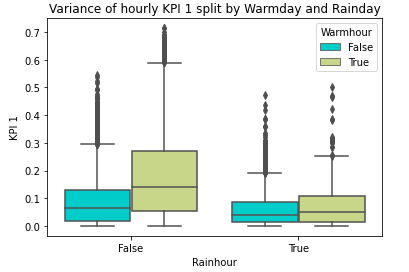
\includegraphics[width=0.8\linewidth]{./Figures/APP1.png}
    \caption{Variance of hourly RPUB split by Warmday and Rainday}
    \label{APP1}
\end{figure}

\begin{figure}[H]
   \centering
    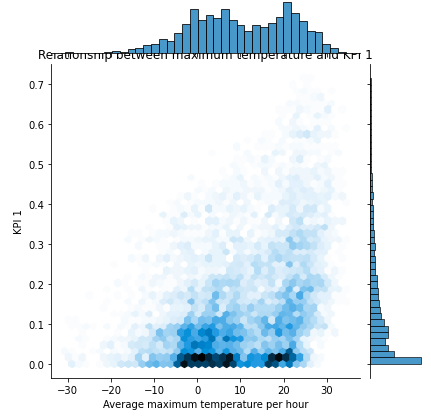
\includegraphics[width=0.8\linewidth]{./Figures/APP2.png}
    \caption{Relationship between maximum temperature and RPUB}
    \label{APP2}
\end{figure}

Investigating a jointplot illustrating the relationship between maximum temperature and RPUB with unique yearly bikes, a linear positive correlation between the average maxi-mum daily temperature and the RPUB (thus, bike usage) can be exhibited. However, the his-togram of RPUB values is comparably equally distributed, being slightly skewed towards low values.

\subsection{KPI 2: Demand-Capacity}
\label{app:A4}

\begin{figure}[H]
   \centering
    \includegraphics[width=0.8\linewidth]{./Figures/kpi2abb2.png}
    \caption{Average hourly KPI 2 value grouped by month}
    \label{kpi2abb2}
\end{figure}

\begin{figure}[H]
   \centering
    \includegraphics[width=0.8\linewidth]{./Figures/kpi2abb3.png}
    \caption{Average hourly KPI 2}
    \label{kpi2abb3}
\end{figure}

\subsection*{More thorough investigation of Demand-Capacity}
\label{app:A2}

\begin{figure}[H]
   \centering
    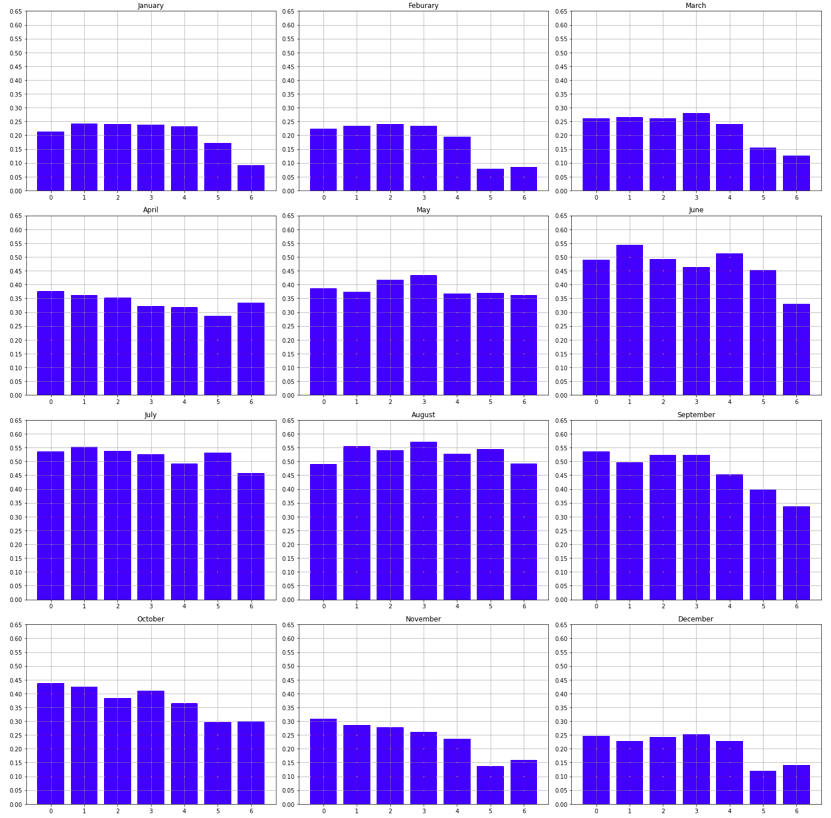
\includegraphics[width=0.8\linewidth]{./Figures/APP1_1.png}
    \caption{Average Demand-Capacity per day per month}
    \label{APP1-1}
\end{figure}

The illustration above depicts the avergage demand-capacity value per day per month. This stresses the notion that was already gained in the main part of this assignment in a sense, that the figures do not, on average, come close to a problematic value of 1.


\subsection{KPI 3: Average Rental Durations}
\label{app:A5}

\begin{figure}[H]
   \centering
    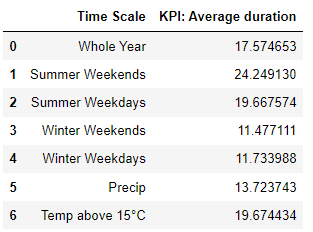
\includegraphics[width=0.4\linewidth]{./Figures/Duration_Fig_2.png}
    \caption{Results KPI 3 Average Rental Durations}
    \label{Duration_Fig_2}
\end{figure}

\subsection{KPI 4: Revenue}
\label{app:A6}

\begin{figure}[H]
    \centering
    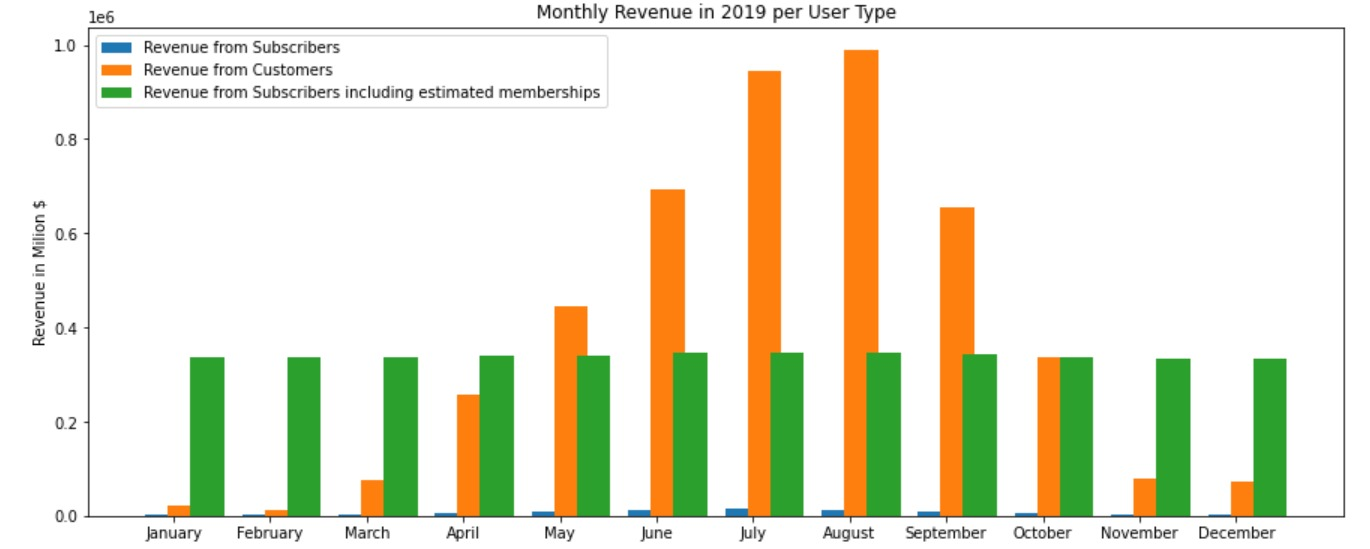
\includegraphics[width=0.9\linewidth]{./Figures/Revenue_monthlyUserType.jpeg}
    \caption{Monthly Revenue in 2019 per User Type}
    \label{fig_revenue_2}
\end{figure}

\begin{figure}[H]
    \centering
    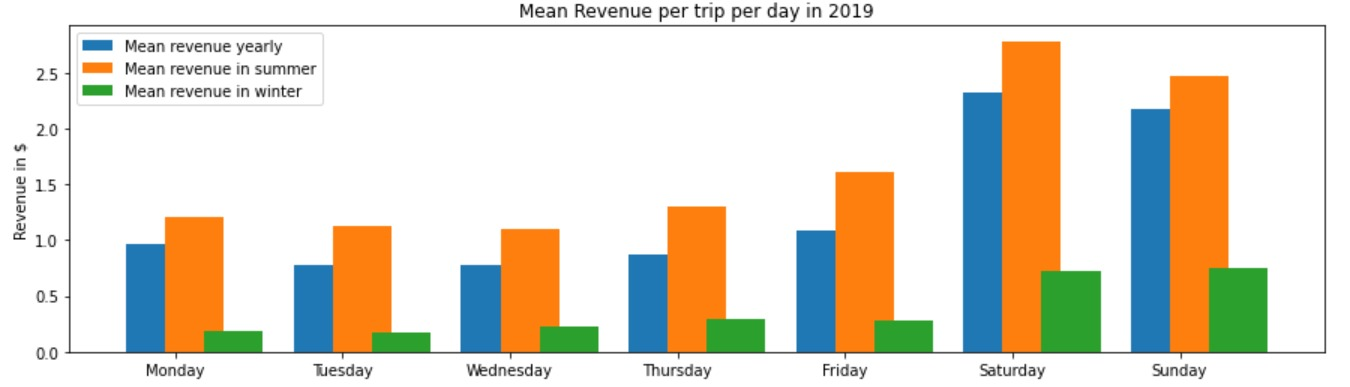
\includegraphics[width=0.9\linewidth]{./Figures/Revenue_week.jpeg}
    \caption{Mean Revenue per trip per day in 2019}
    \label{fig_revenue_3}
\end{figure}

\subsection{Cluster Analysis}
\label{app:A7}

\begin{figure}[H]
   \centering
    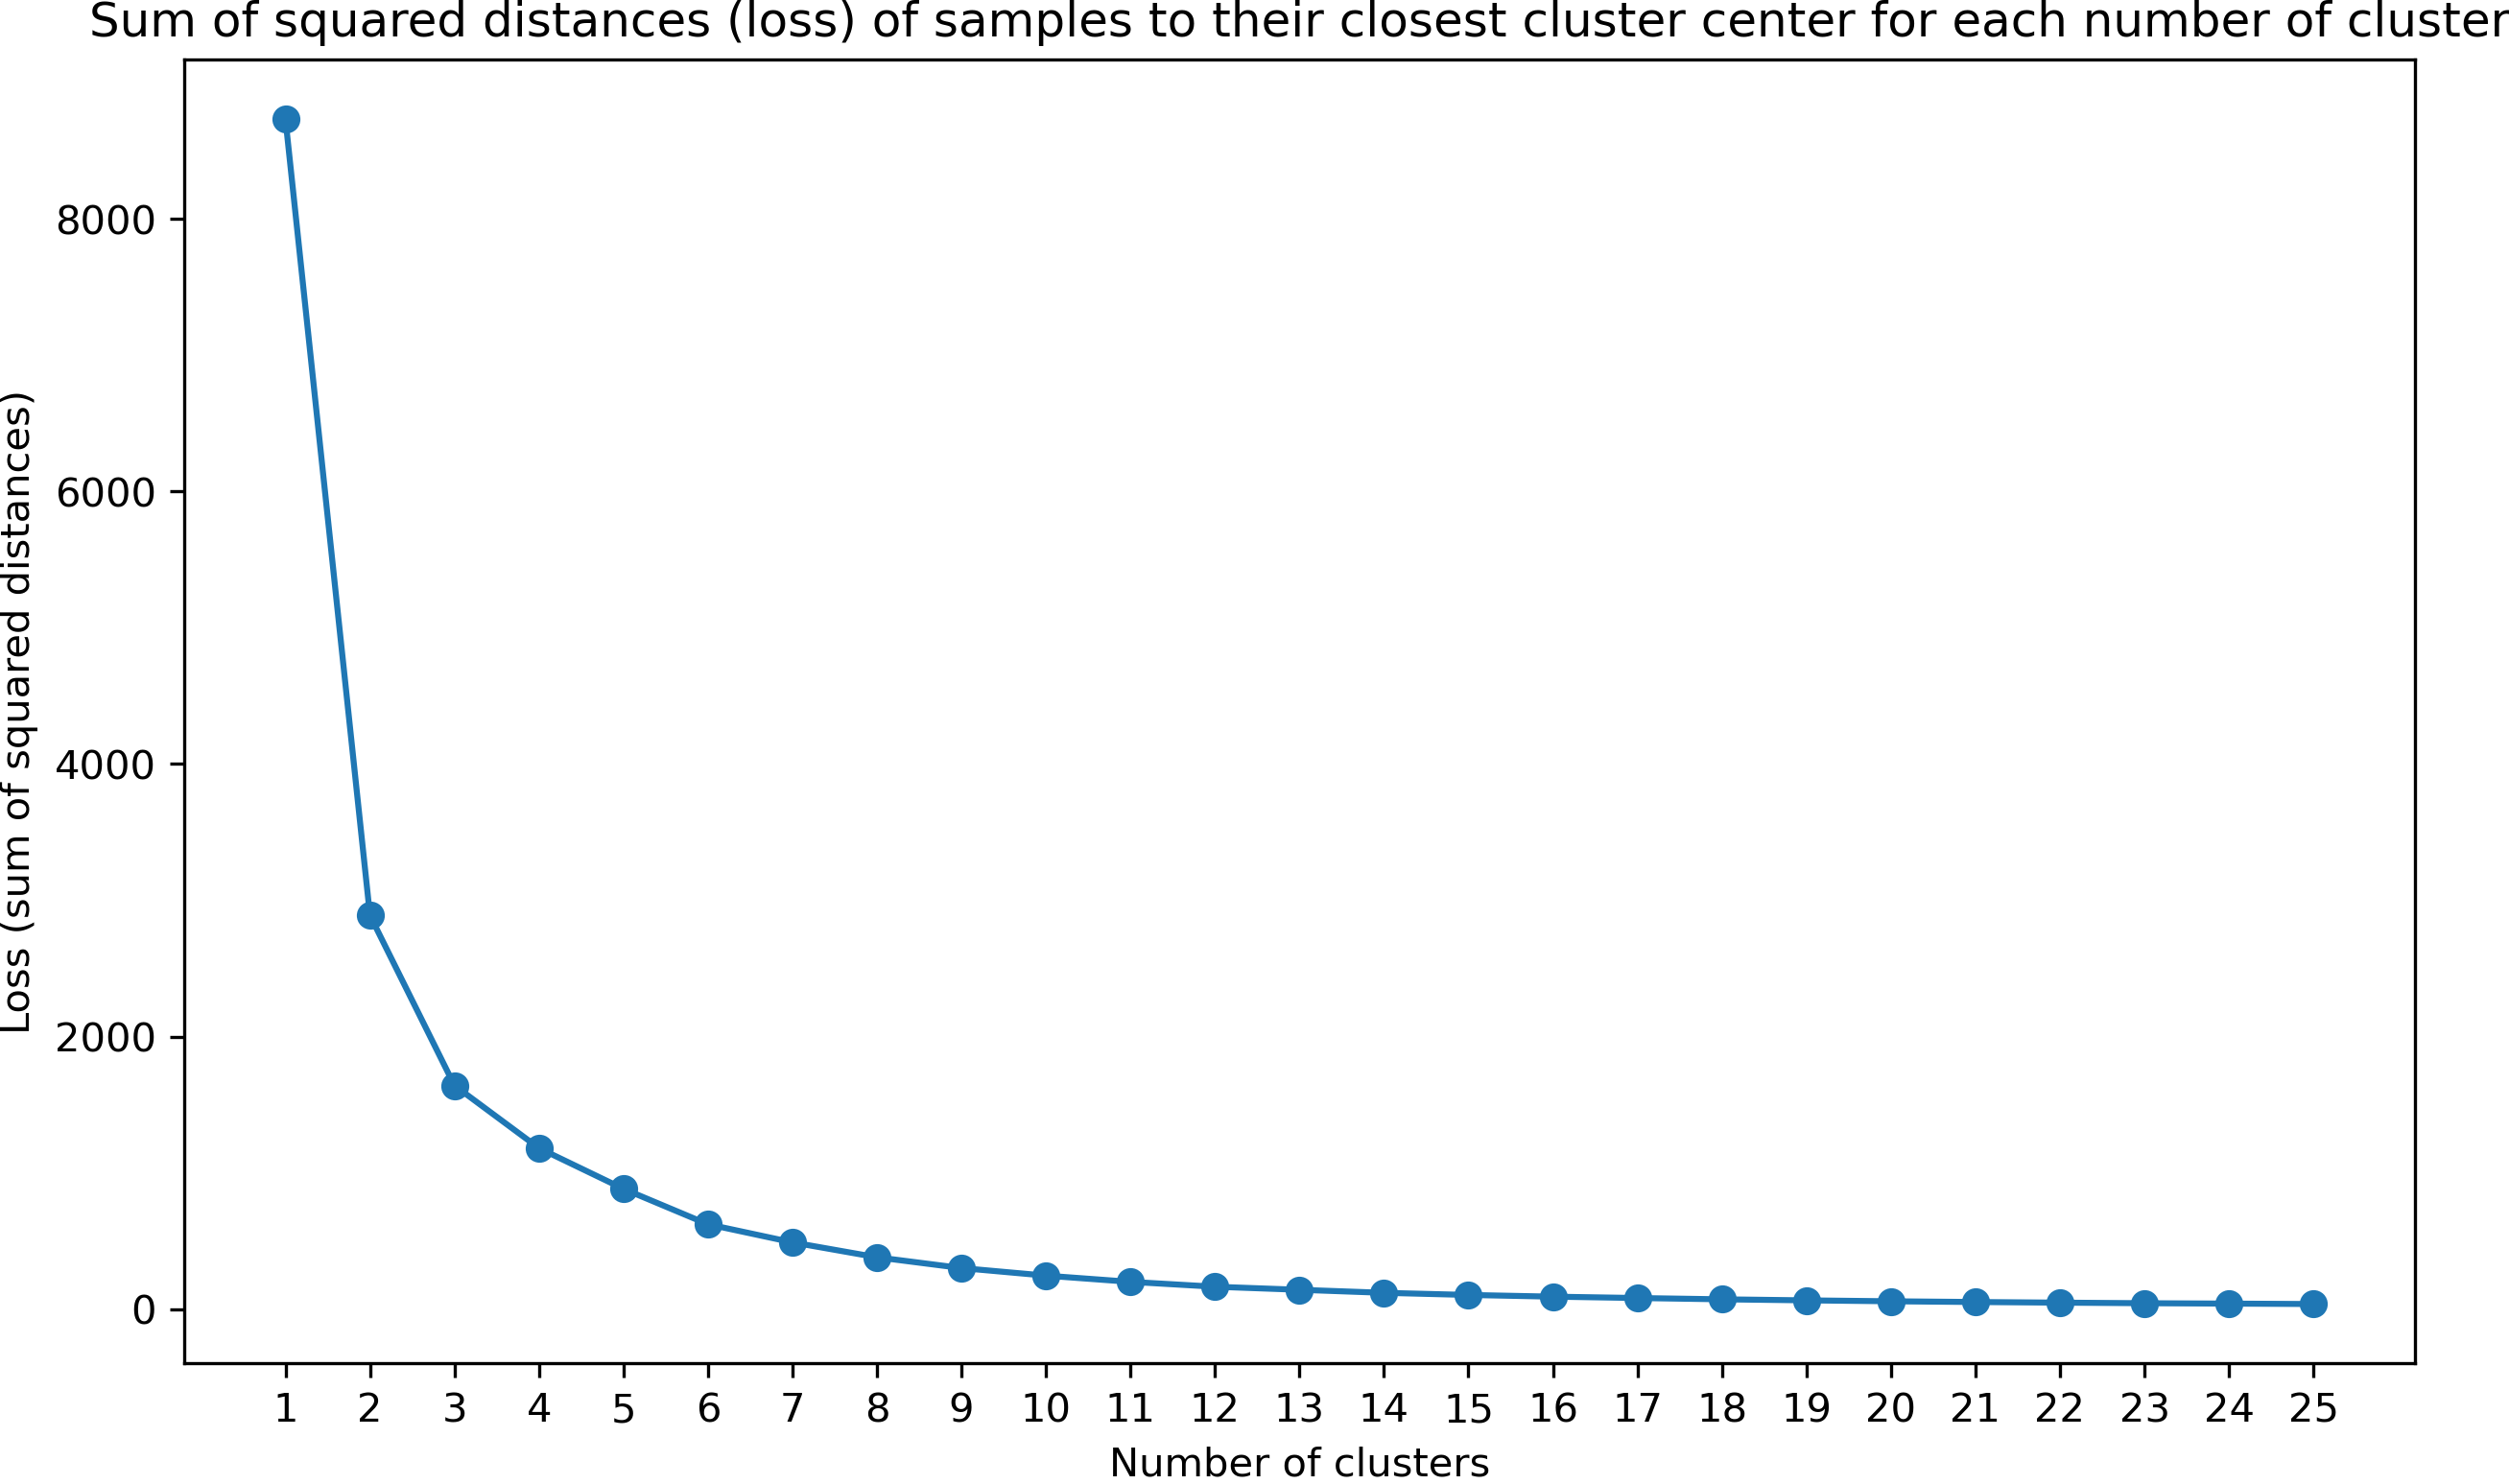
\includegraphics[width=0.8\linewidth]{./Figures/LossKMeans_Duration_dpi300.png}
    \caption{Sum of squared distances (loss) of samples to their closest cluster center for each number of cluster for duration}
    \label{LossKMeans_Duration_dpi300}
\end{figure}

\begin{figure}[H]
   \centering
    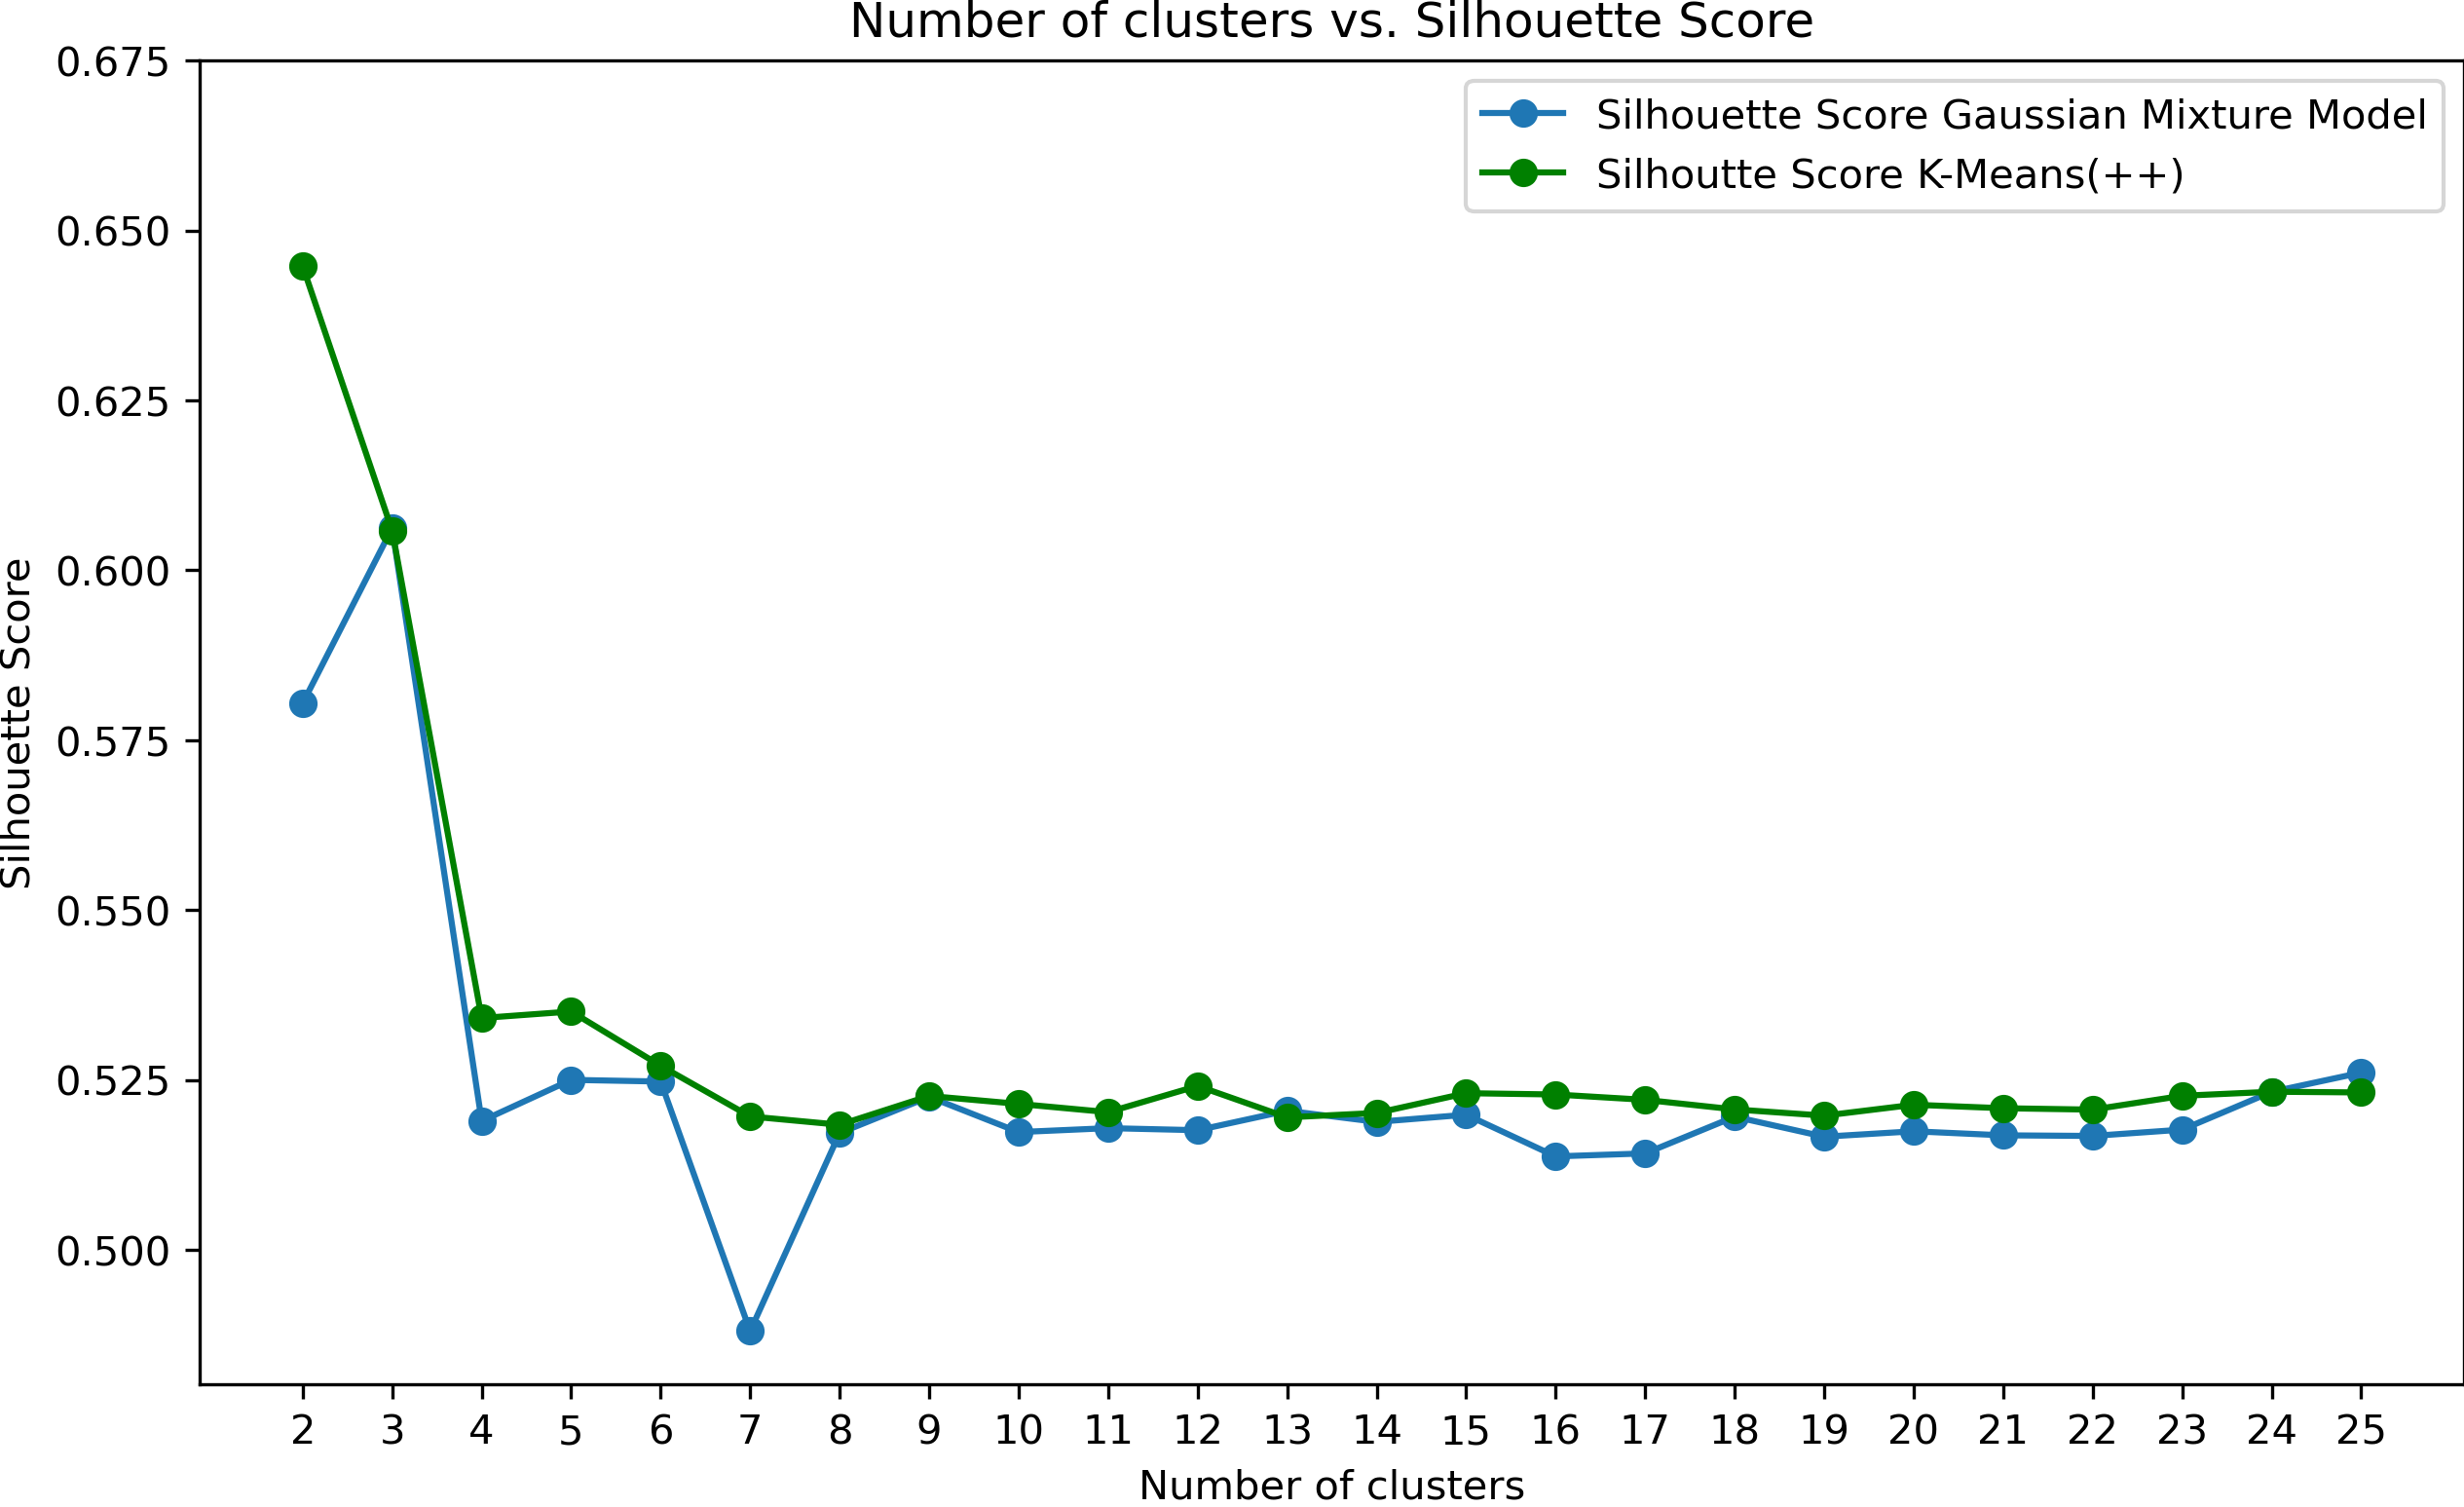
\includegraphics[width=0.8\linewidth]{./Figures/Silhouette_Duration.png}
    \caption{Silhouette score for each number of clus-ter for duration}
    \label{Silhouette_Duration}
\end{figure}

\begin{figure}[H]
   \centering
    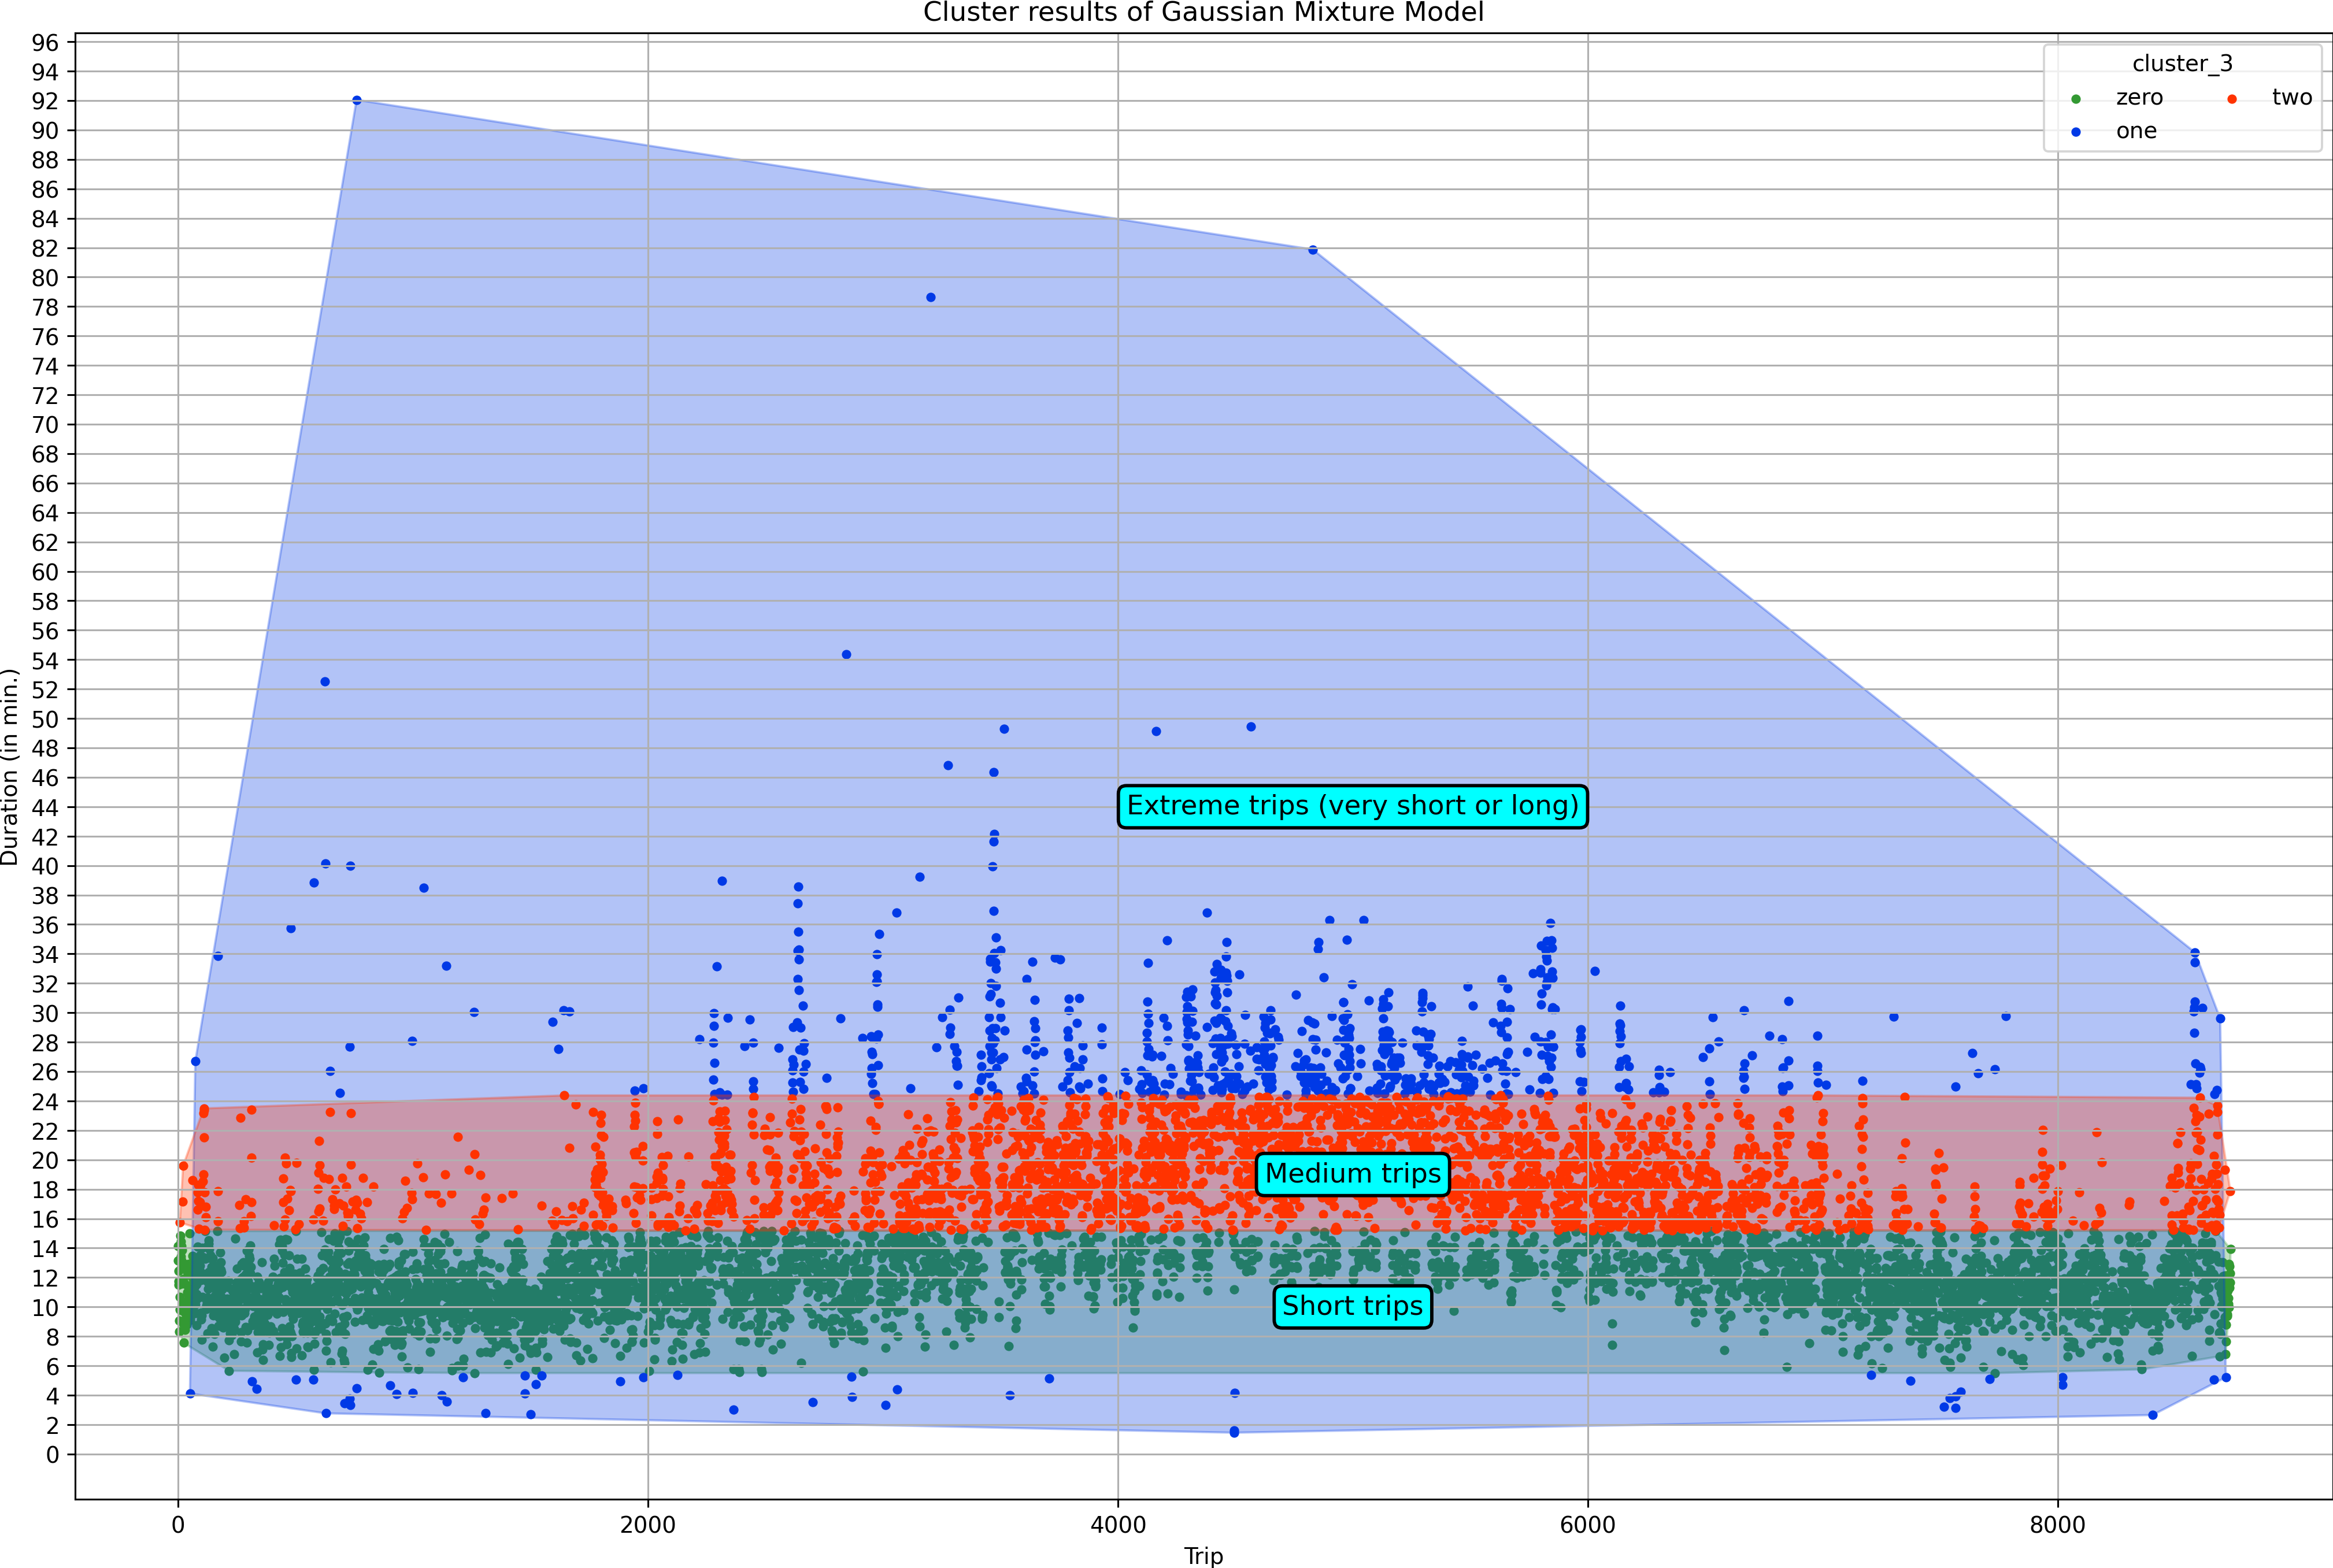
\includegraphics[width=0.8\linewidth]{./Figures/FINAL_Cluster_Gaussian_Duration.png}
    \caption{Cluster results of Gaussian Mixture Model}
    \label{FINAL_Cluster_Gaussian_Duration}
\end{figure}

\begin{figure}[H]
   \centering
    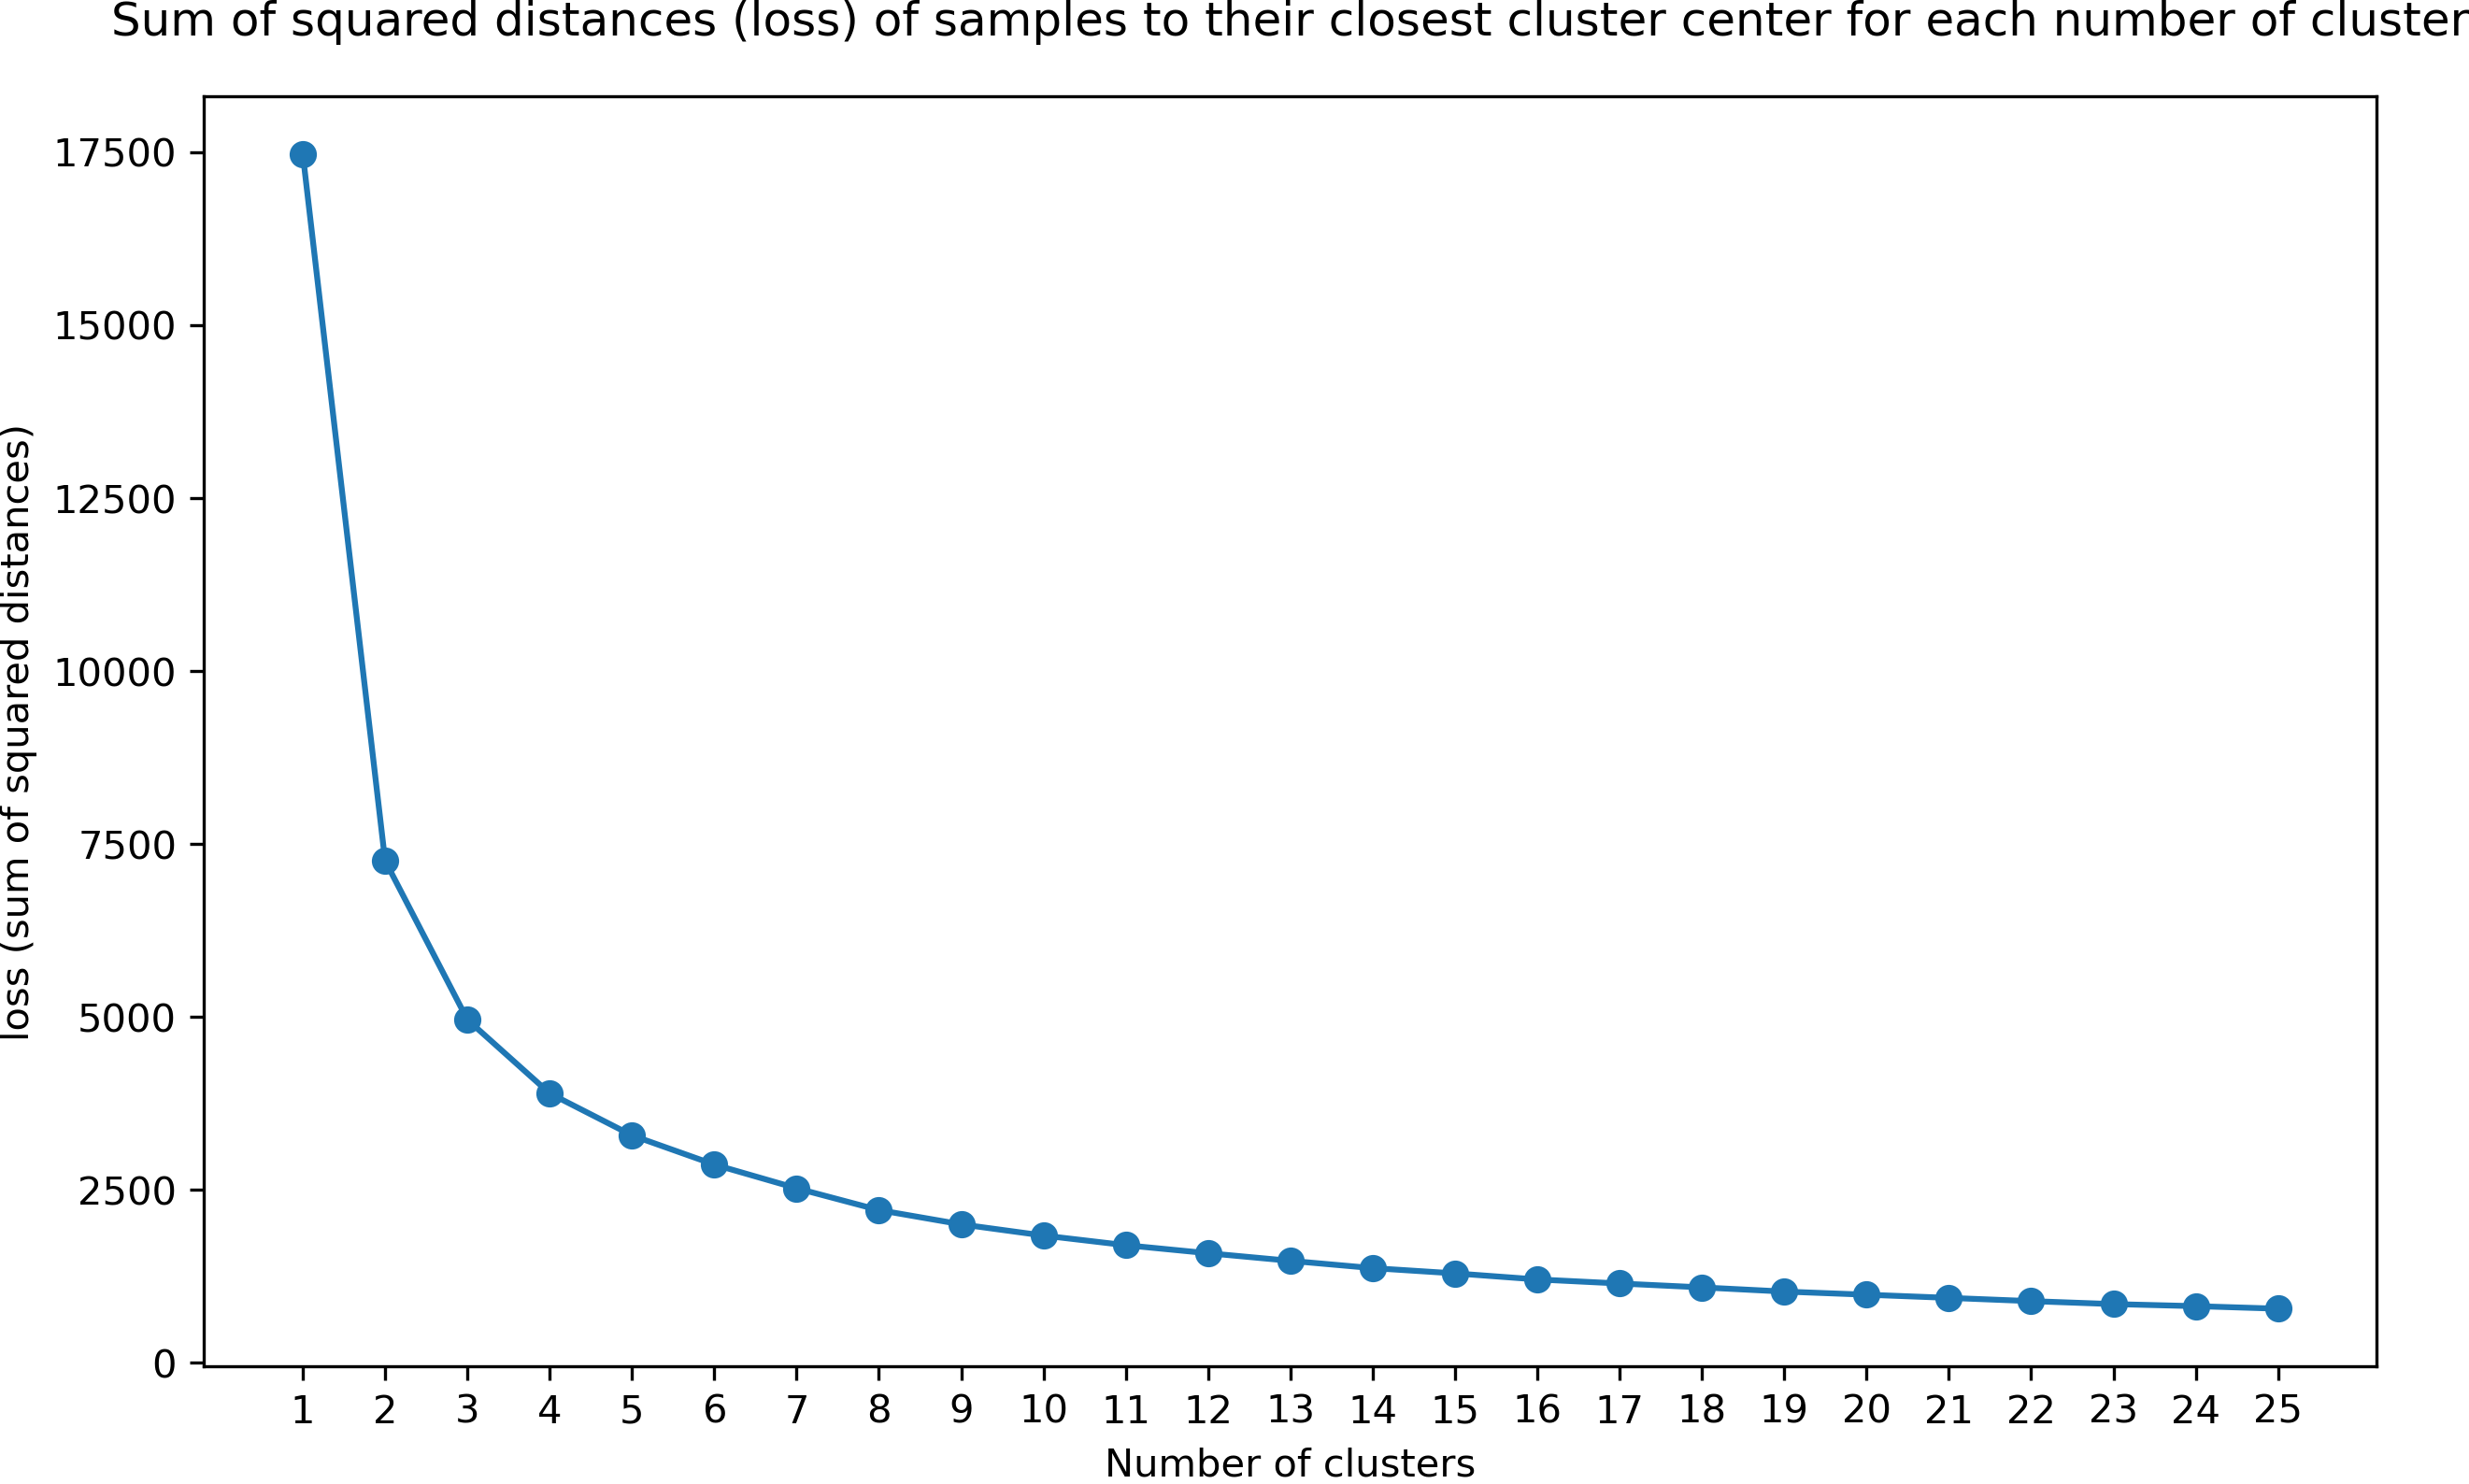
\includegraphics[width=1\linewidth]{./Figures/Loss_Duration_Temp.png}
    \caption{Sum of squared distacnes (loss) of samples to their closet cluster center for each number of cluster (duration and temperature)}
    \label{Loss_Duration_Temp}
\end{figure}

\begin{figure}[H]
   \centering
    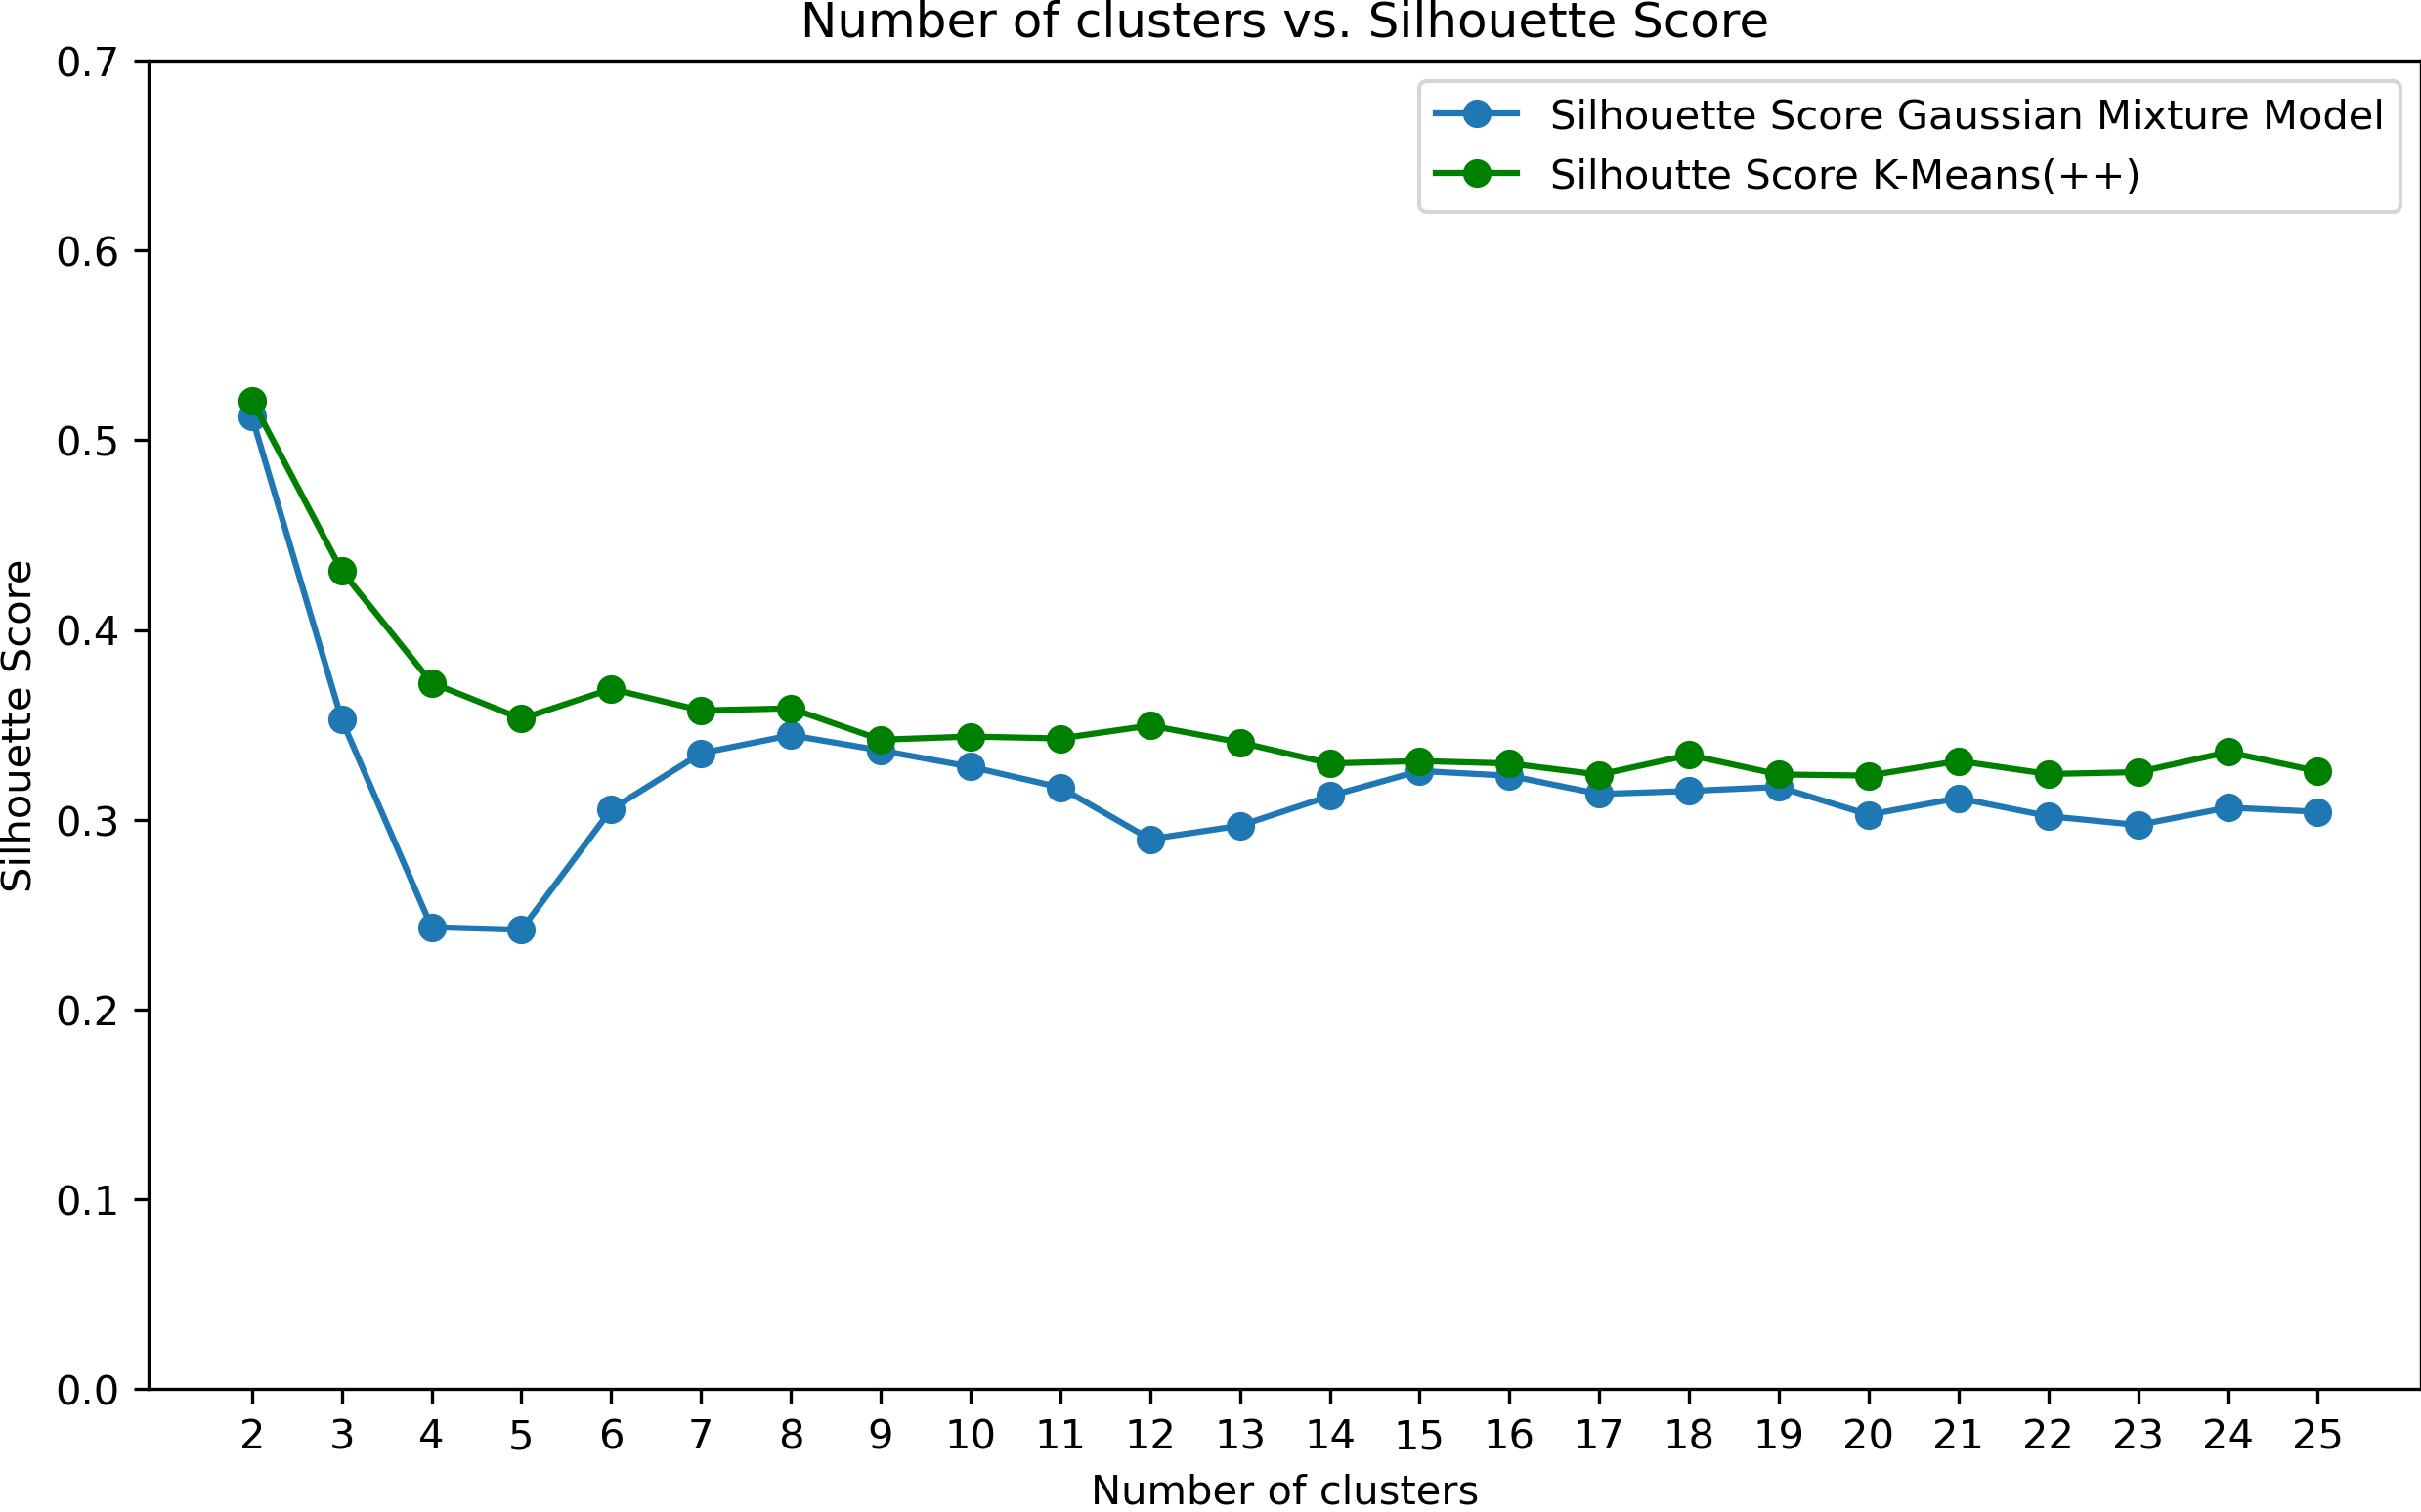
\includegraphics[width=1\linewidth]{./Figures/Silhouette_Gaussian_Duration_Temp.png}
    \caption{Number of clusters vs. Silhouette Score (duration and temperature)}
    \label{Silhouette_Gaussian_Duration_Temp}
\end{figure}

\begin{figure}[H]
   \centering
    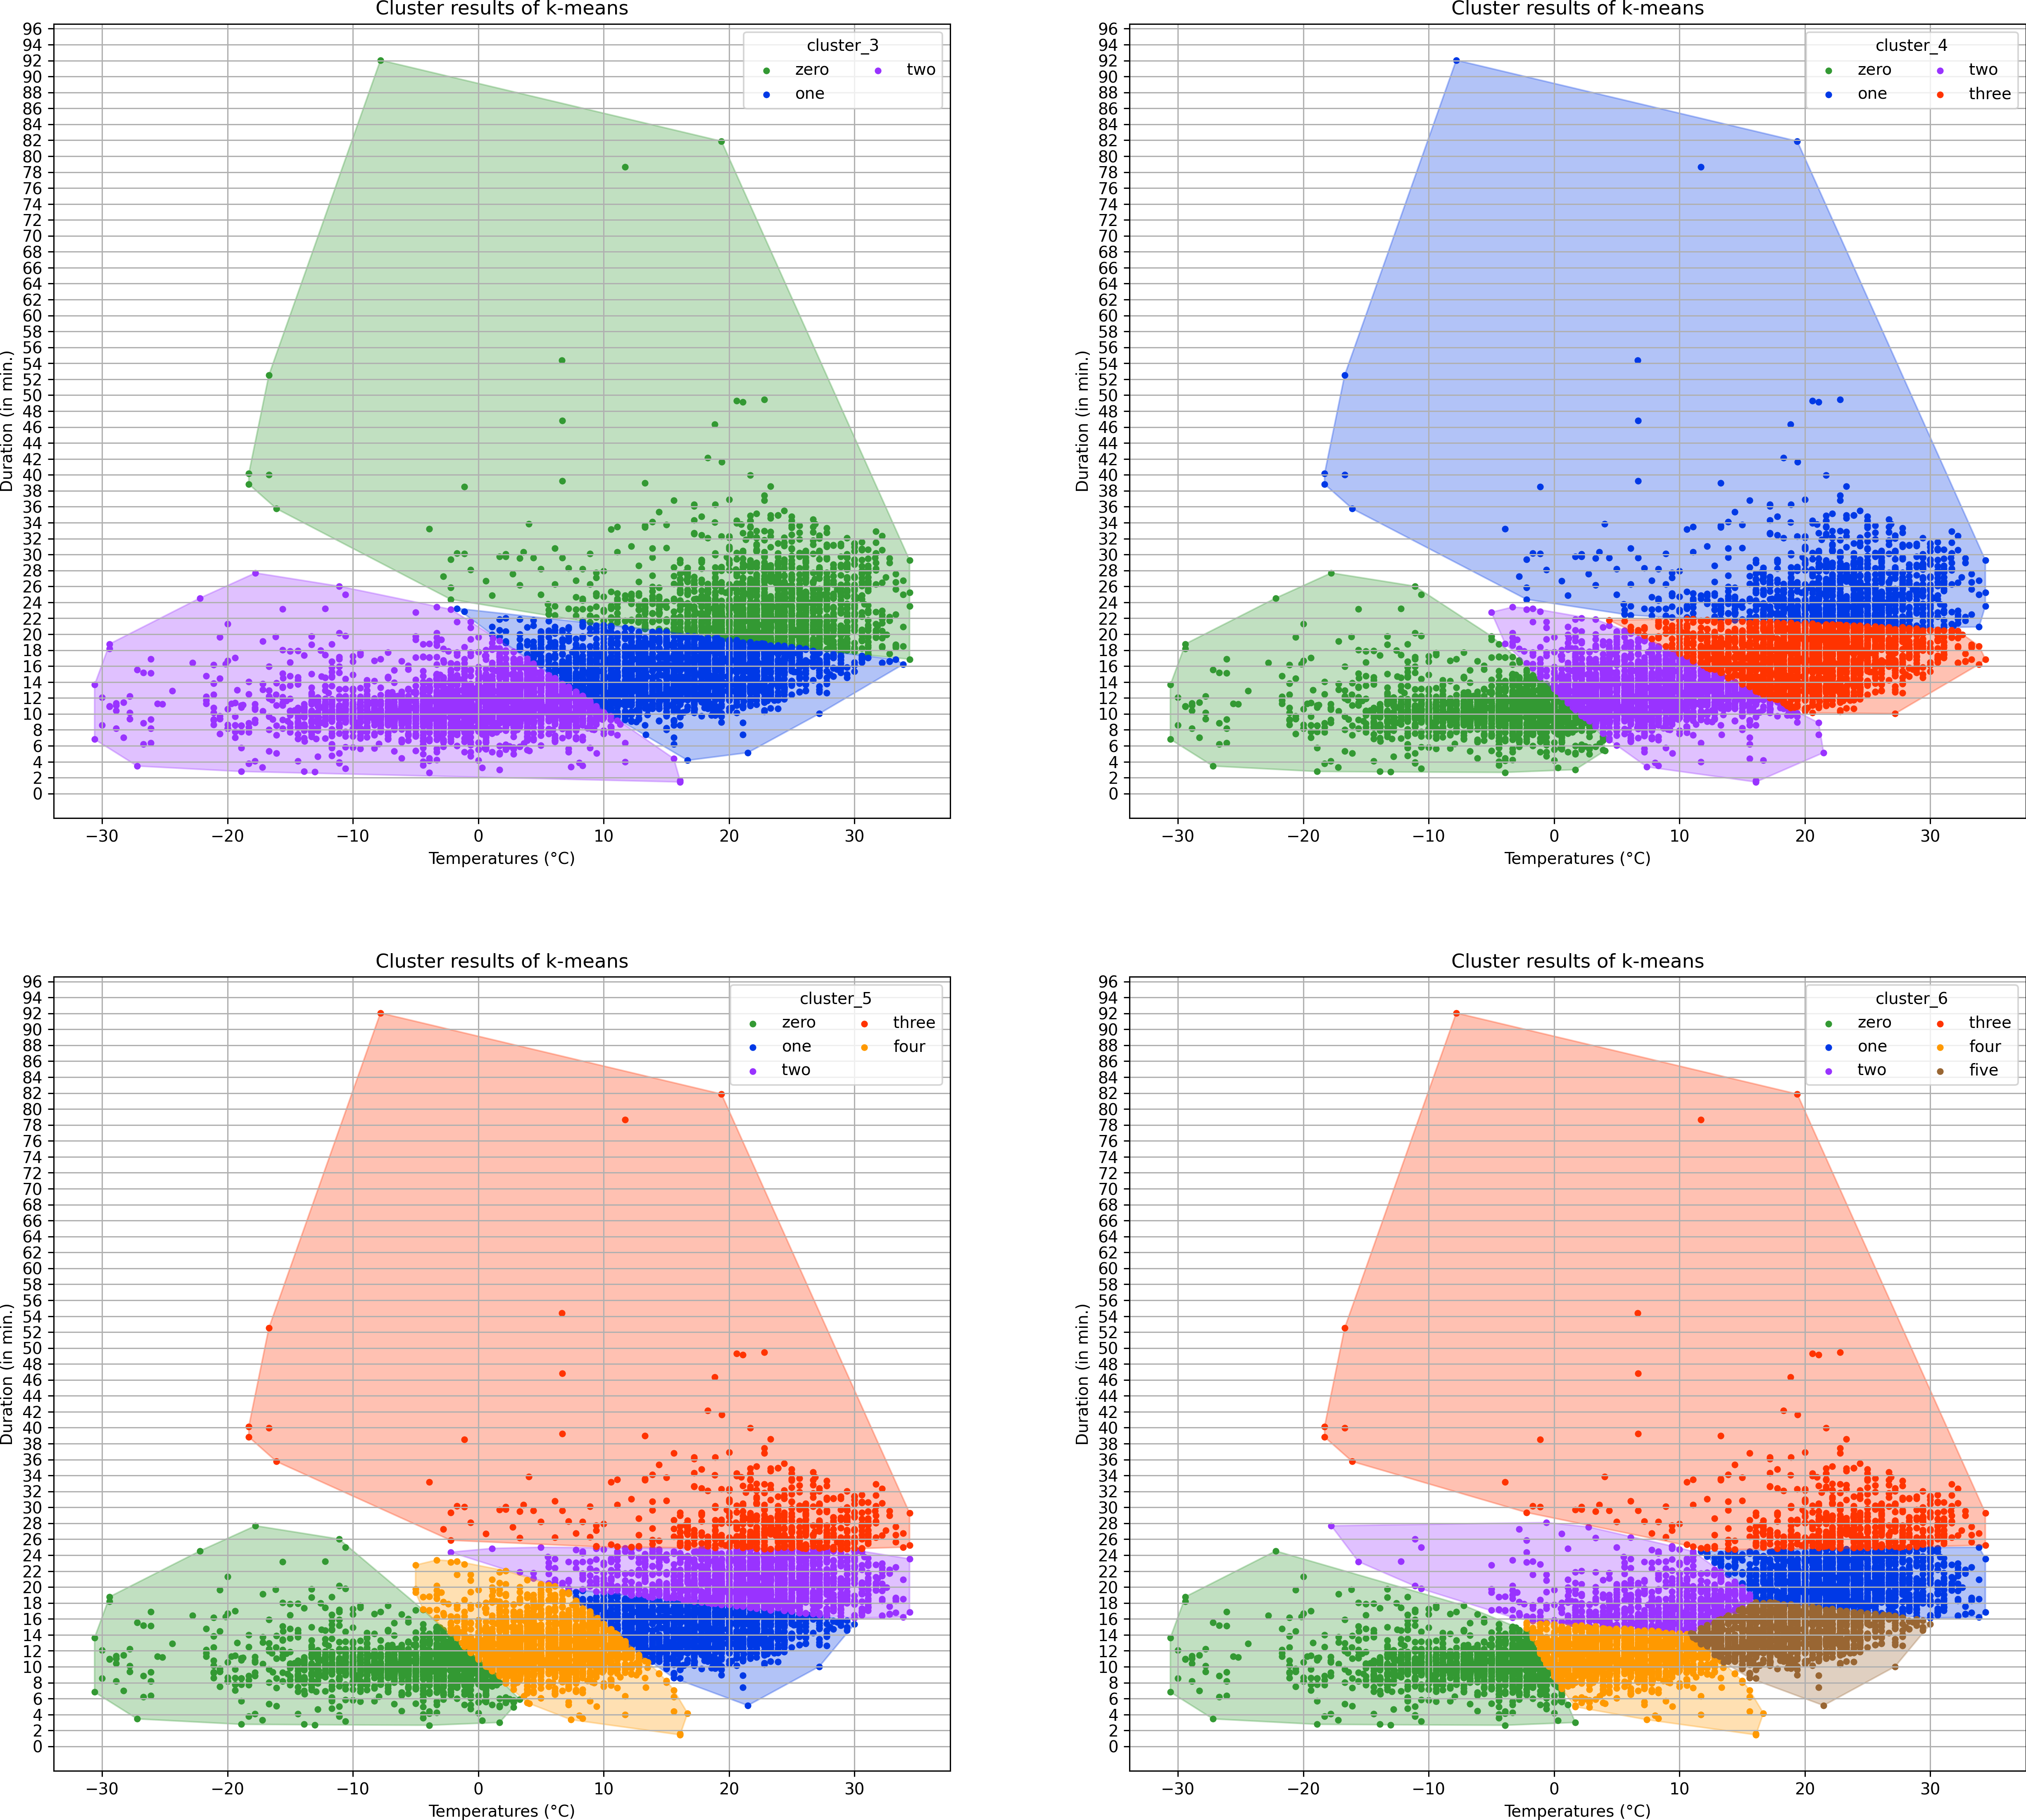
\includegraphics[width=1\linewidth]{./Figures/Cluster_KMEANS_Duration_Temp.png}
    \caption{Cluster results K-Means - duration and temperature}
    \label{Cluster_KMEANS_Duration_Temp}
\end{figure}

\begin{figure}[H]
   \centering
    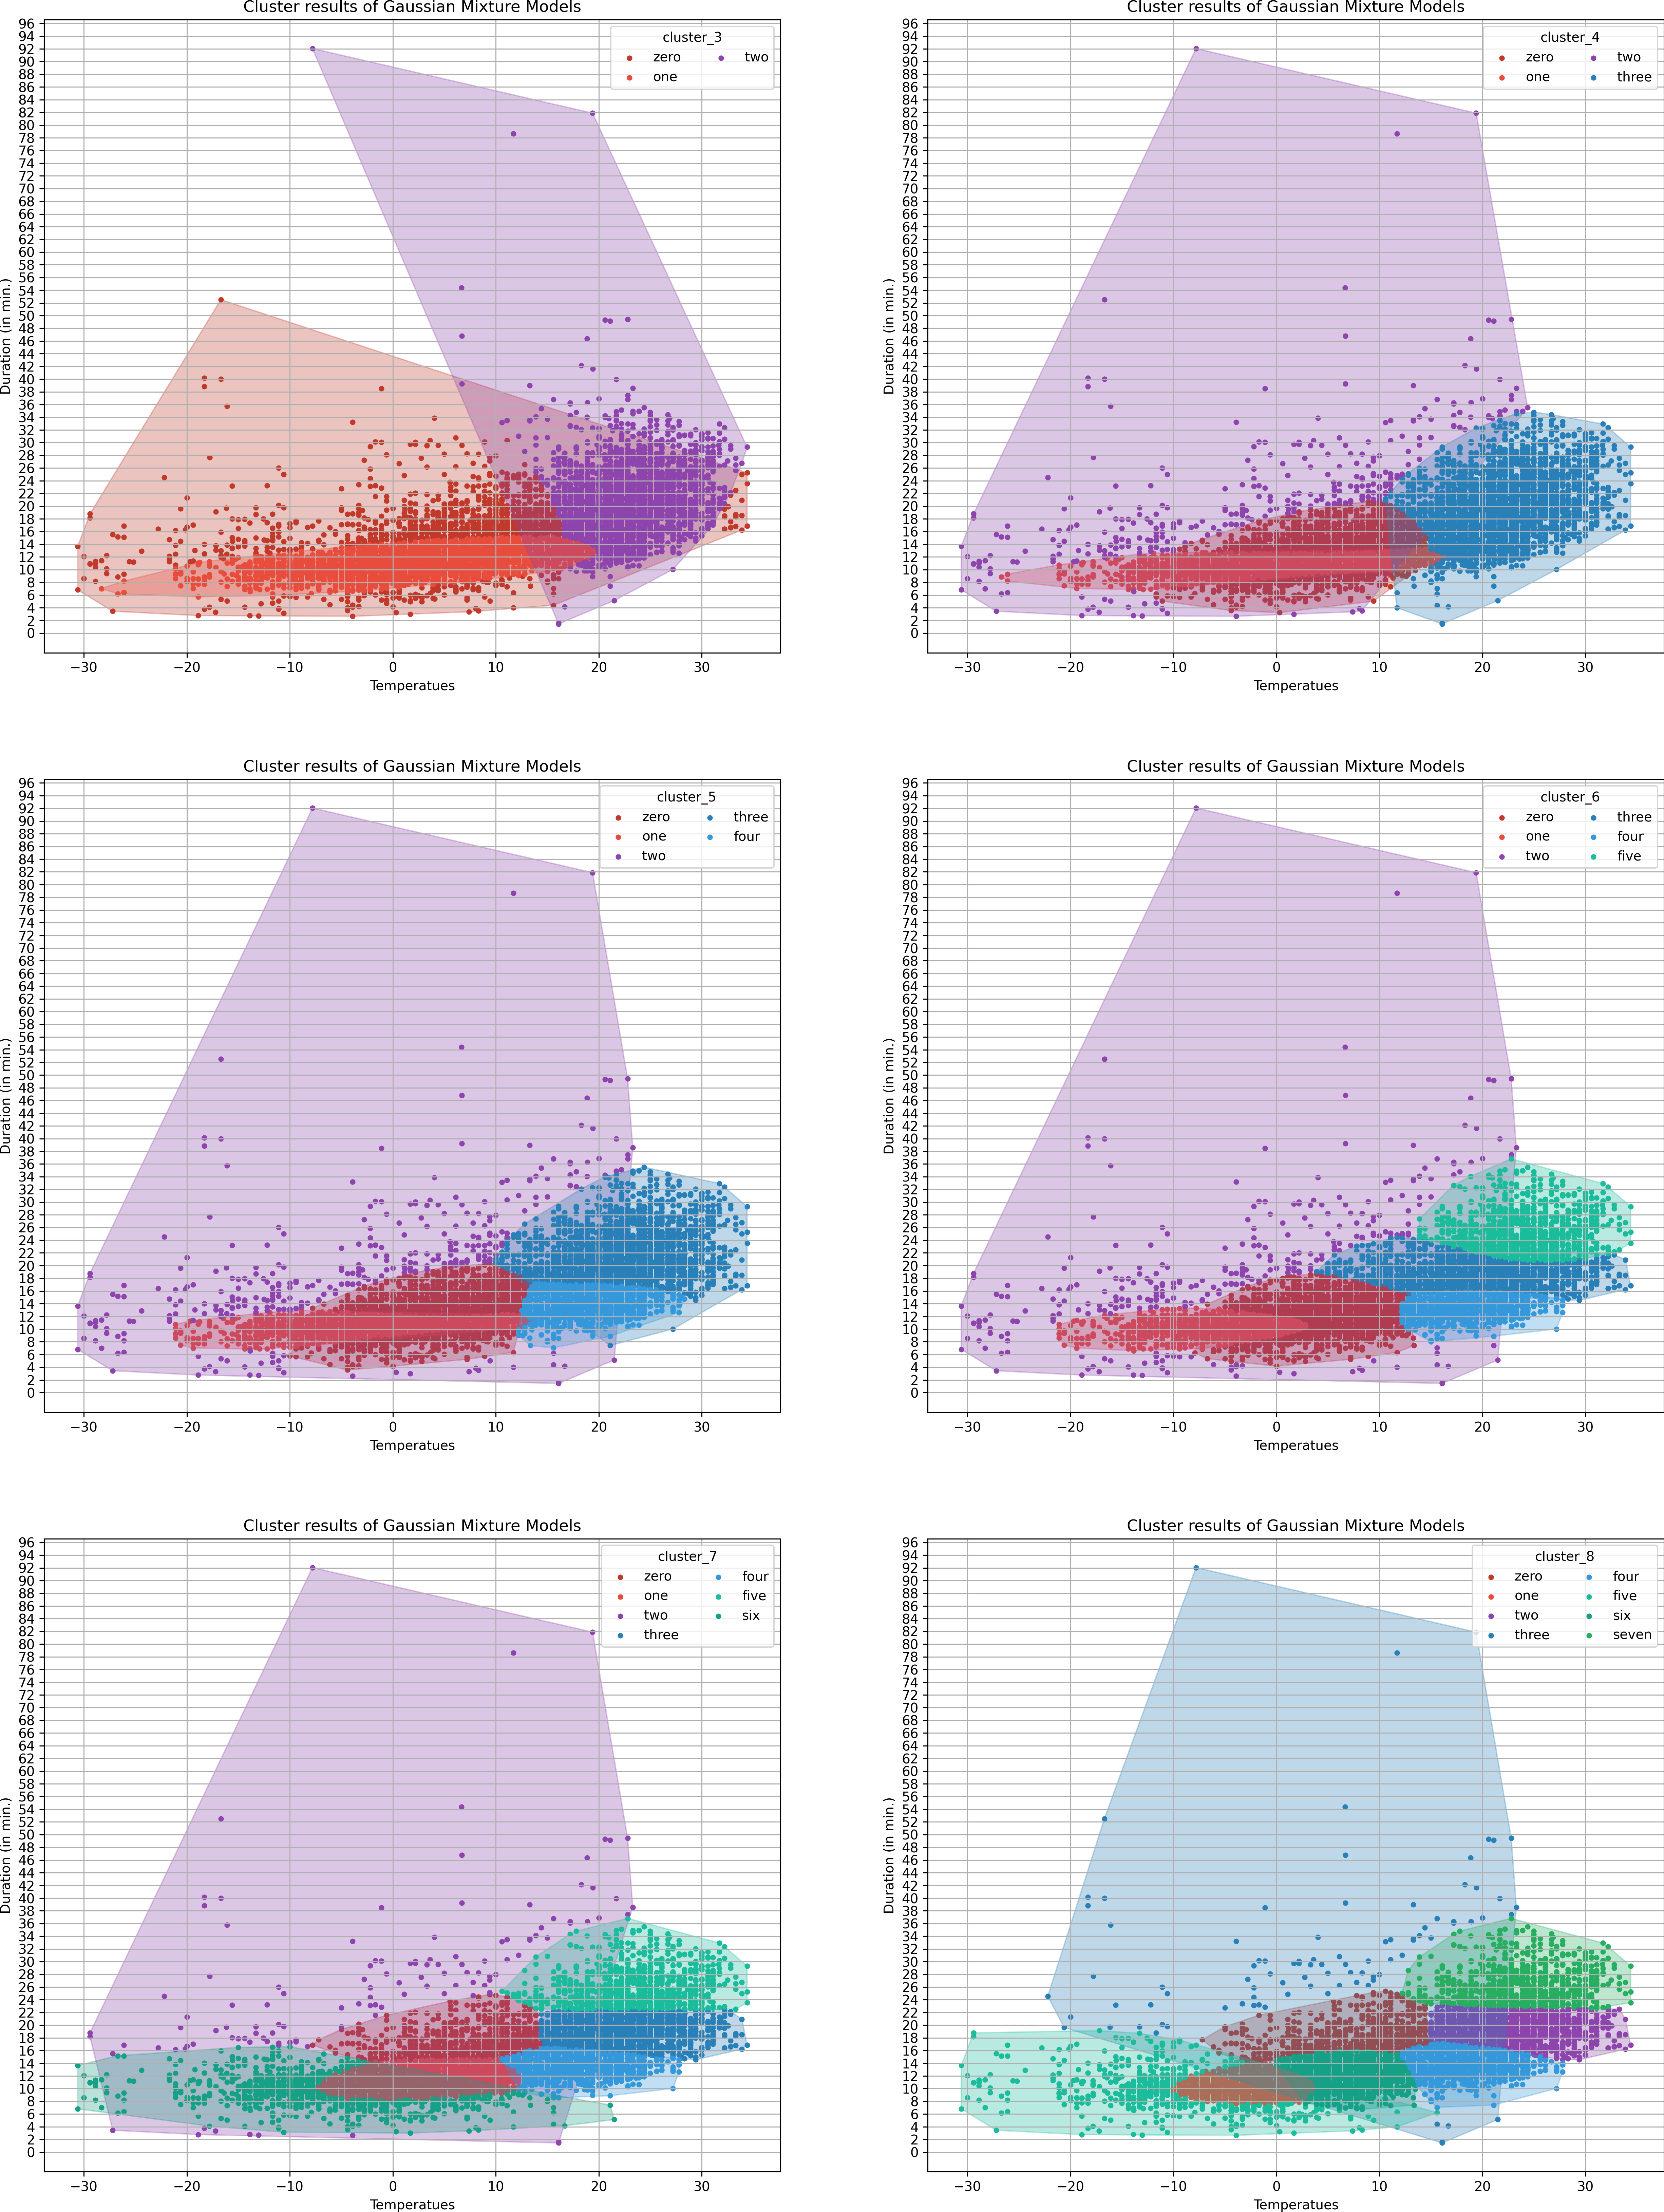
\includegraphics[width=1\linewidth]{./Figures/Clusters_Gaussian_Duration_Temp.png}
    \caption{Cluster results Gaussian Mixture Model - duration and temperature}
    \label{Clusters_Gaussian_Duration_Temp}
\end{figure}

\begin{figure}[H]
   \centering
    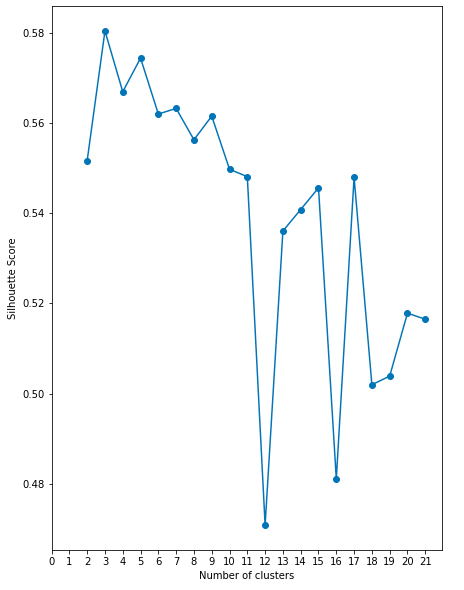
\includegraphics[width=0.8\linewidth]{./Figures/BC_ABB1.png}
    \caption{Silhouette score for clustering based on demand-capacity}
    \label{BCABB1}
\end{figure}

\subsection*{Revenue Clustering using K-Means}
\label{app:A3}

\begin{figure}[H]
   \centering
    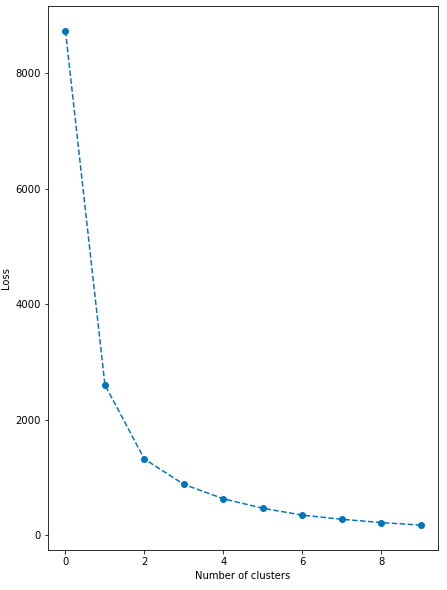
\includegraphics[width=0.8\linewidth]{./Figures/BC_APP1.png}
    \caption{Optimal number of clusters using K-Means instead of GMM}
    \label{BCAPP1}
\end{figure}

\begin{figure}[H]
   \centering
    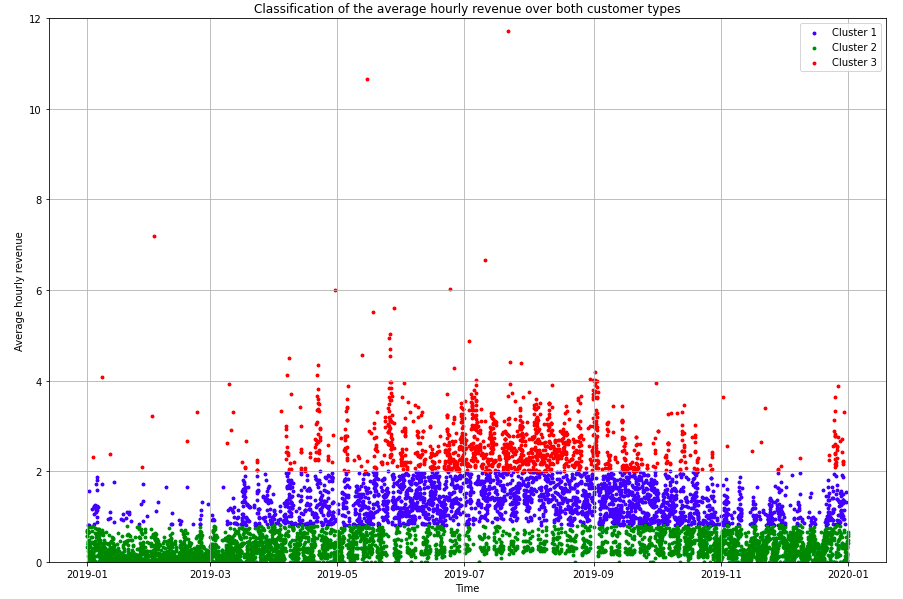
\includegraphics[width=0.8\linewidth]{./Figures/BC_APP2.png}
    \caption{Clustering of the Average Hourly Revenue over both Customer Types using K-Means}
    \label{BCAPP2}
\end{figure}

Comparing the here depicted results of K-Means and GMM in the main part, the green layer here is larger. As we consider this to be more realistic (there are often very short rides below 30 minutes that create only low revenue) we continued to work with the clustering created by Guten Morgen Mamachen! in the main section.


\begin{figure}[H]
   \centering
    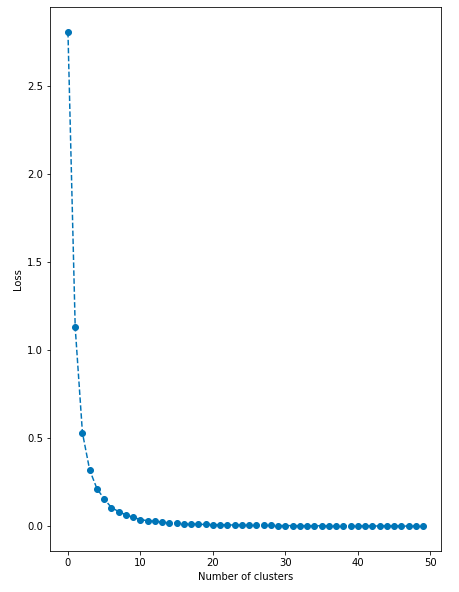
\includegraphics[width=0.8\linewidth]{./Figures/BC_ABB7.png}
    \caption{Optimal Number of Clusters Attempt (individual stations)}
    \label{BCABB7}
\end{figure}

\subsection*{Clustering based on Revenue and Average Hourly Station Temperature}
\label{app:A4}

\begin{figure}[H]
   \centering
    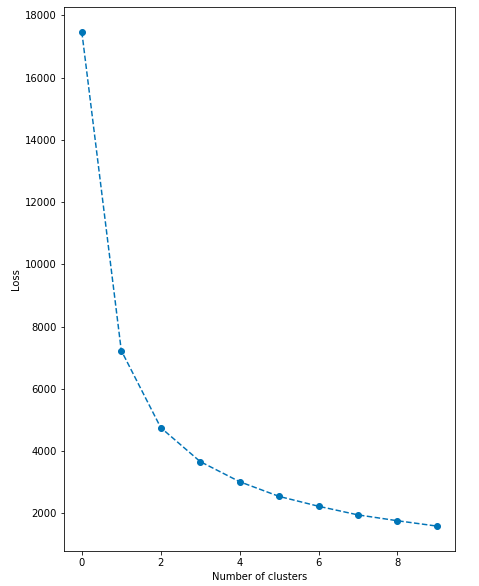
\includegraphics[width=0.8\linewidth]{./Figures/BC_APP5.png}
    \caption{Optimal number of clusters}
    \label{BCAPP5}
\end{figure}

\begin{figure}[H]
   \centering
    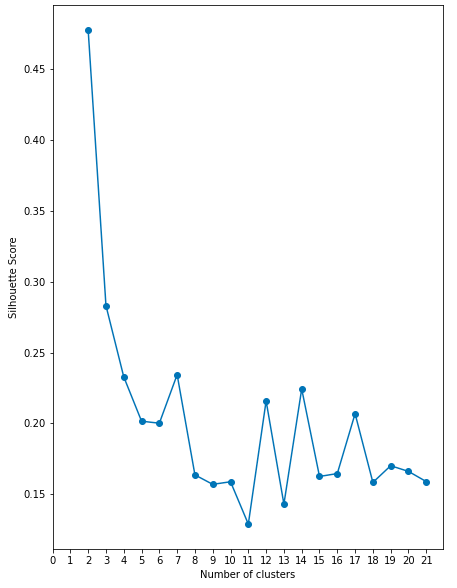
\includegraphics[width=0.8\linewidth]{./Figures/BC_APP6.png}
    \caption{Silhouette score for clustering based on demand-capacity}
    \label{BCAPP6}
\end{figure}

When we add the average hourly temperature as an input feature, K-Means again yields that 3 clusters are optimal (APP 5). GMM indicated an optimum of 2 clusters (APP 6), which we decided was too low and thus, GMM are inappropriate. 

\begin{figure}[H]
   \centering
    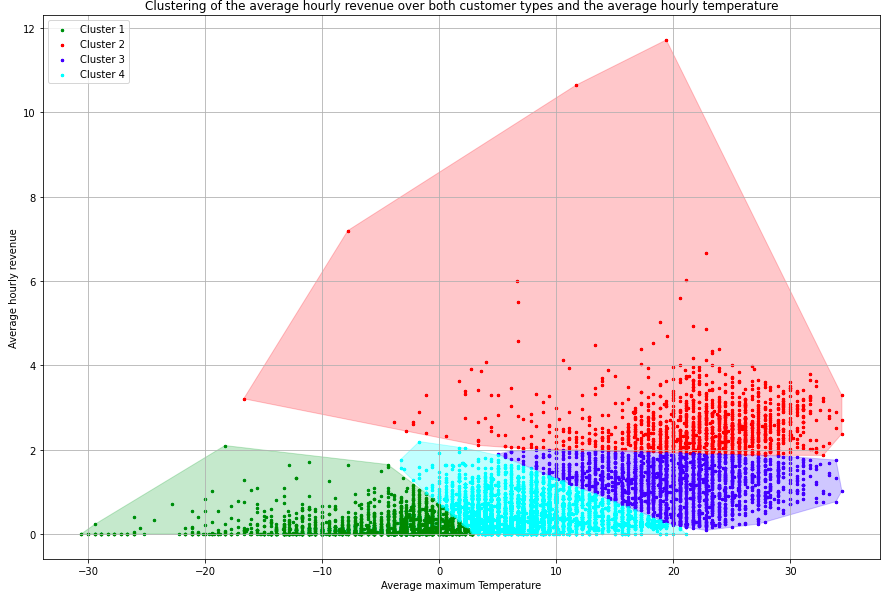
\includegraphics[width=0.8\linewidth]{./Figures/BC_APP7.png}
    \caption{Clustering of the average hourly revenue over both customer types and the average hourly temperature}
    \label{BCAPP7}
\end{figure}

Investigating the results of the K-Means clustering (APP 7), the green, cyan and blue clusters exhibit roughly the same reve-nue and are mainly distinguished by the average maximum temperature per respective hour. The red cluster exhibits the highest average hourly revenue, together with the highest vari-ance in terms of average hourly temperature, although, as it is to expect, the data points are nevertheless skewed towards temperatures above 0 degrees.

\subsection*{Clustering based on Revenue and Average Yearly Demand-Capacity Value}
\label{app:A5}

\begin{figure}[H]
   \centering
    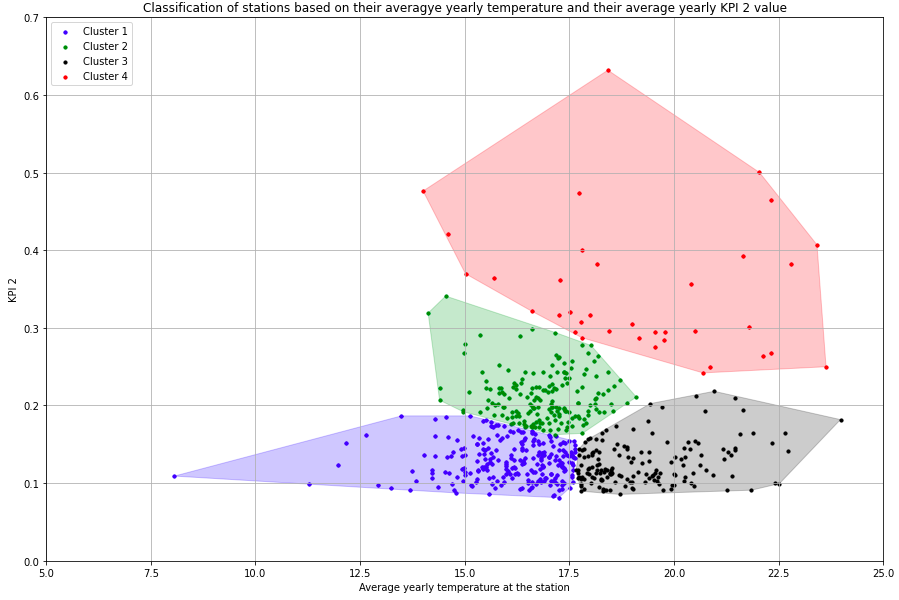
\includegraphics[width=0.8\linewidth]{./Figures/BC_APP8.png}
    \caption{Classification of stations based on their average yearly temperature and their average yearly KPI2 value}
    \label{BCAPP8}
\end{figure}

Our goal is to try to further differentiate the (former/above described) green and blue clusters to see if any new patterns can be derived. Therefore, we add another feature - the average yearly temperature per station that was present when a ride started. In terms of Demand-Capacity, again three layers arise. However, the lowest layer (black and blue), while exhibiting roughly the same distribution in terms of Demand-Capacity, shows a significant difference in terms of the average temperature of starting rides there. The red cluster is pretty predominant in terms of both temperature and Demand-Capacity.

\begin{figure}[H]
   \centering
    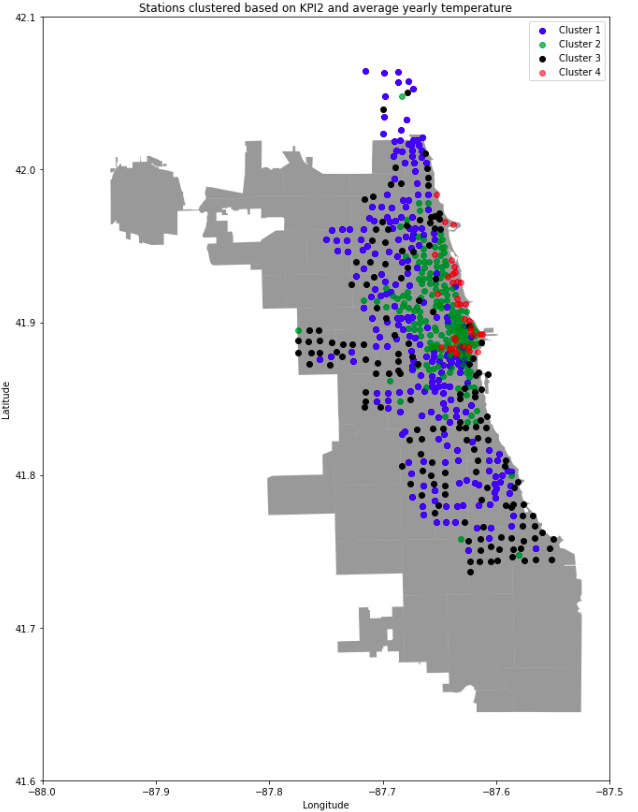
\includegraphics[width=0.8\linewidth]{./Figures/BC_APP9.png}
    \caption{Stations clustered based on KPI2 and average yearly temperature}
    \label{BCAPP9}
\end{figure}

Interestingly, although we now implemented four clusters, the general structure derived from only taking Demand-Capacity into account remains steady: We still see highly used stations around the lake and two large rings around them. The red stations are still situated mainly around parks etc. and at one small cluster downtown, just as above. However, the "outskirt" stations were differentiated by adding another cluster. While occasionally, there are some areas where black stations are predominant and others where blue stations are predominant, no real dif-ferentiation can be made. Thus, average yearly ride starting temperature does not seem to be a very good way to further distinguish the stations.

\subsection*{Clustering based on the total number of starting rides per station}
\label{app:A7}

\begin{figure}[H]
   \centering
    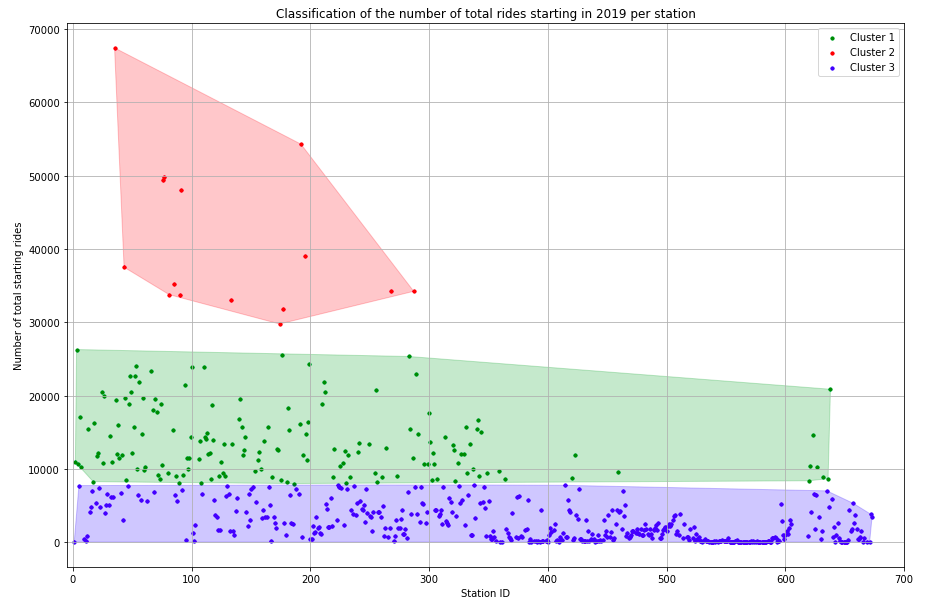
\includegraphics[width=0.8\linewidth]{./Figures/BC_APP10.png}
    \caption{Classification of the number of total rides startig in 2019 per stations}
    \label{BCAPP10}
\end{figure}

We will introduce an alternative to the Demand-Capacity for two reasons. Firstly, Demand-Capacity is relatively com-plex conceptually and thus not that easy to understand. Secondly, we want to gain a different perspective and see, what clusters arise then. Thus, we will simply use the total number of starting rides per station over the year 2019 as input feature here.
The red cluster stands slightly out as the difference of the distribution of the number of start-ing rides for that cluster is higher than the difference between the blue and the green cluster.

\begin{figure}[H]
   \centering
    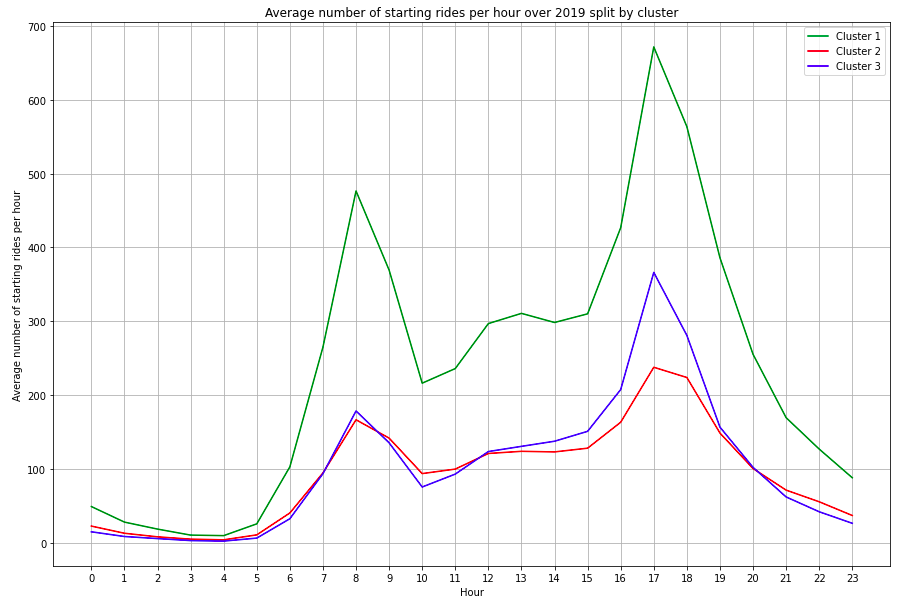
\includegraphics[width=0.8\linewidth]{./Figures/BC_APP11.png}
    \caption{Average number of starting rides per hour over 2019 split by cluster}
    \label{BCAPP11}
\end{figure}

In the graph above we plot the average number of starting rides per hour over the year 2019. Clearly and as already observed in the descriptive part of the assignment, the commuter pat-tern can be seen - all three graphs peak at around 8 and 17 o' clock, respectively. Interest-ingly, comparing the blue and the red cluster, it becomes clear that both peaks for the red cluster are roughly the same value, while the 17 o' clock peak for the blue cluster is signifi-cantly higher than the 8 o'clock peak. However, it is difficult to deduce something related to the type of trips/customers based solely on that observation. Interestingly, although the red clustered stations above account for the highest number of starting rides, the "mediocre" cluster in green stands out significantly in the figure below.

\begin{figure}[H]
   \centering
    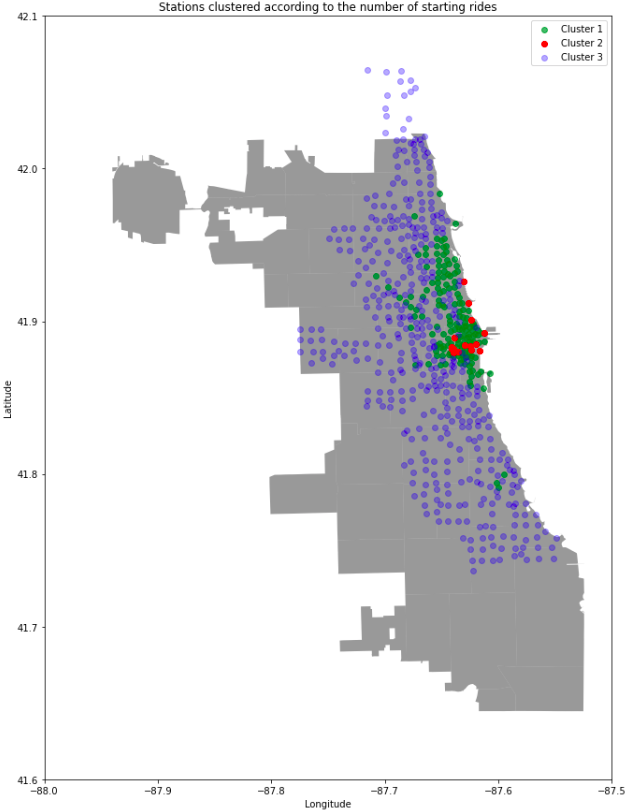
\includegraphics[width=0.8\linewidth]{./Figures/BC_APP12.png}
    \caption{Stations clustered according to the number of starting rides}
    \label{BCAPP12}
\end{figure}

Interestingly, when creating the same geospatial plot as above (then based on Demand-Capacity values), the number of red stations seems to be smaller, however the sites were those are located is similar to the clustering based on Demand-Capacity. The blue stations seem to be predominant compared to the green ones and the diffusion of those two station types does not be as high as based on Demand-Capacity. This might be due to the fact that Demand-Capacity dissects the different activities on each sta-tion more thoroughly and thus yields a more specific, distinguishable image. Nevertheless, the three-ring-structure as above can still be observed. Hence, both Demand-Capacity and the number of starting rides per station yield, overall, the same distribution of stations and thus, seem to be reasonable measures.

\begin{figure}[H]
   \centering
    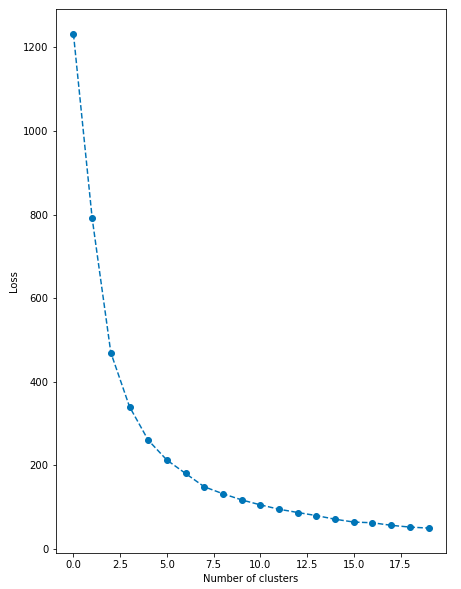
\includegraphics[width=0.7\linewidth]{./Figures/BC_ABB11.png}
    \caption{Optimal Numbers of Clusters for numer of starting rides per station and average duration}
    \label{BCABB11}
\end{figure}

\subsection{Predictive Analysis}
\label{app:A8}

\begin{figure}[H]
   \centering
    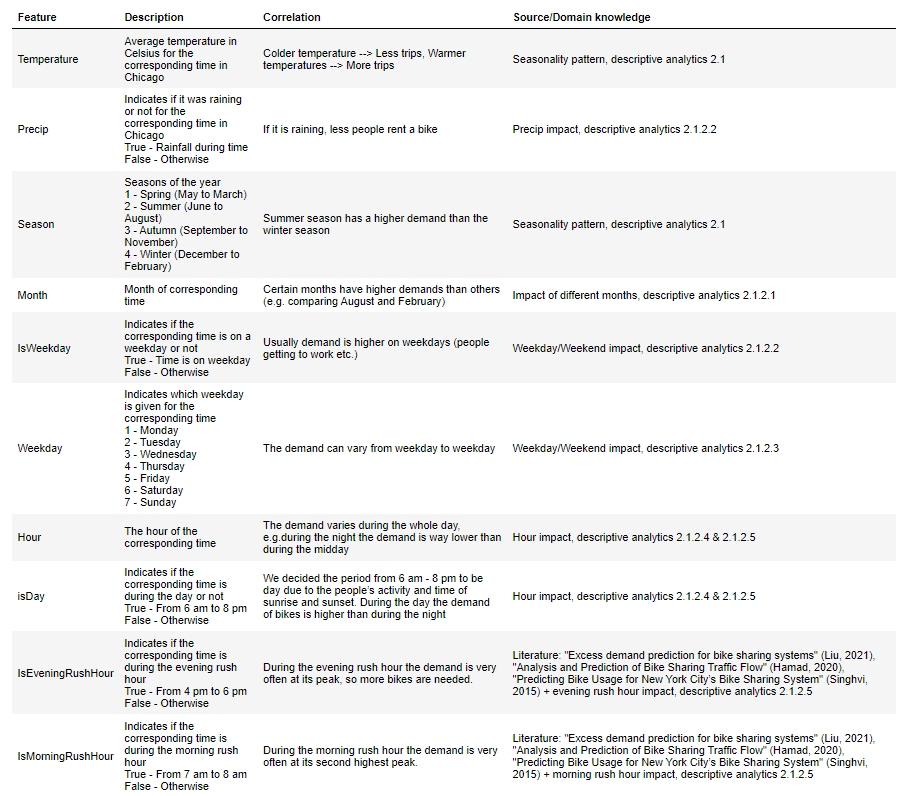
\includegraphics[width=1\linewidth]{./Figures/RF_Fig_1.png}
    \caption{Developed Features}
    \label{Pred_Fig_1}
\end{figure}

\begin{table}[H]
\begin{tabular}{p{0.2\textwidth}p{0.2\textwidth}p{0.1\textwidth}p{0.4\textwidth}}
    \toprule
    \textbf{Hyperparameter} & \textbf{Description }  & \textbf{Final Value} & \textbf{Interpretation} \\
    \midrule
    Bootstrap & Boolean if bootstrap samples are used & True & Bootstrap is used, i.e. that the trees are not fitted on all available data but on data subsets which can reduce the variance  \\
    \hline
    Alpha & Parameter for regulating the tree size & 0.6 & Relatively high value, meaning that there is a larger penalty on the tree size \\
    \hline
    Max Depth  & Maximum depth of three, meaning how many levels of nodes it can have & 90 & A tree size of 90 seems relatively high, and overfitting could occur, but the alpha parameter regulates this   \\
    \hline
    Max Features & Maximum number of features to split at each node & 5 & For each split 5 random features of our dataset, which comprises 6 in total, are looked at. In CART all features are taken into account, as CART use a greedy algorithm. However, this results in structural similar trees and as we know ensemble methods work best if the sub-models are uncorrelated. Taking 5 features reduces this problem.\\
    \hline
    Min Samples Leaf & Minimum number of samples required in a leaf node & 1 & One sample in the leaf means that the tree could be recursively partitioned until each sample is in one leaf. This would overfit the data, however the max depth and min samples split reduce that risk\\
     \hline
     Min Samples Split & Minimum number of samples needed to split a node & 3 & In order to split a node, a minimum number of 3 samples is needed. This can reduce the generalization error, as the tree can not split until each leaf only has one sample.\\
     \hline
     Estimators & Number of trees on which the prediction is calculated based on mean computation & 250 & 250 decision trees are used, which lies in the typical range of 100 to 1.000 trees and should be sufficient for generalizable prediction\\
    \bottomrule
\end{tabular}
\caption{\label{table:basti}Bastian 1}
\end{table}



\begin{table}[H]
\centering
\begin{tabular}{p{0.1\textwidth}p{0.1\textwidth}p{0.1\textwidth}p{0.1\textwidth}p{0.1\textwidth}p{0.1\textwidth}}
    \toprule
    \textbf{Model} & \textbf{1}  & \textbf{2} & \textbf{3} &  \textbf{4} & \textbf{5}\\
    \midrule
    R$^{2}$ (in \%)& 74.35 & 95.85 & 98.81 & 98.78 & 98.80  \\
    \hline
    MAE & 158.84 & 119.54 & 76.30 & 74.47 & 74.52  \\\\
   
    \bottomrule
\end{tabular}
\caption{\label{table:basti2}Bastian 2}
\end{table}

\begin{figure}[H]
   \centering
    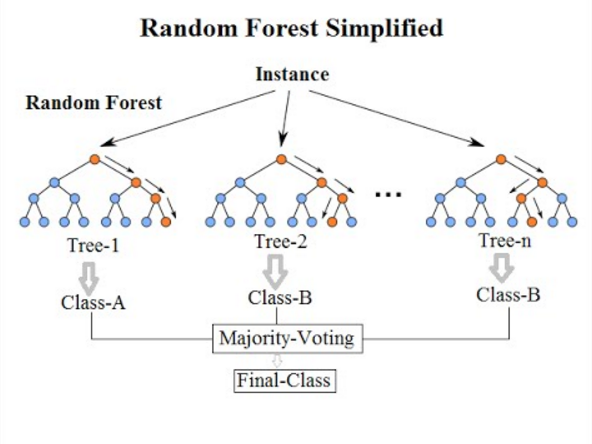
\includegraphics[width=0.8\linewidth]{./Figures/RF_Intro.png}
    \caption{Schematic representation Random Forst}
    \label{RF_Intro}
\end{figure}

\subsection*{Addendum Random Forst: Algorithm and reasons for choosing it}
\label{addendumRF}
As we know that a Random Forest is a composition of several decision trees, we need to understand the decision tree algorithm. In a decision tree for regression, the tree is built top-down from a root node and each node is recursively partitioned into two parts based on the provided features in order to achieve a minimum variance reduction (in classification information gain). On each node level, each feature is looked at and split various times to see how large the variance would be in that new node. Then the idea is to pick the feature and split which maximizes the variance reduction, i.e. which split reduces the variance from parent to child the most. However, if we let the algorithm run to an end, each training target might result in one leaf. This would introduce massive overfitting. To tackle this issue, pruning the tree is necessary. So the pruning process trades off a higher squared error in the validation dataset against the number of decision nodes in the pruned tree to arrive at a tree that captures the patterns but not the noise. This can be done by using cost complexity, which takes both mentioned aspects into account \hyperref[Fig_CC]{Figure XX}. The alpha value can be varied, meaning at alpha = 0 there is no penalty on tree size, while if alpha is getting larger the tree size decreases. The idea here is to start with a full-grown tree and then start to increase alpha gradually until the cost complexity of the full tree exceeds the one of a subtree. This is then repeated until a set of different sized trees and error rates is built. Then one can choose the minimum error tree for a model. The prediction in a leaf is made by taking the average of all instances in that node. On top of this algorithm, a Random Forest has two other hyperparameters (besides these for the decision trees). These are the number of decision trees to calculate the mean computation on and the number of features taking into consideration to split a node. The number of estimators typically lies within a range of 100 to 1.000. Generally speaking, the more trees, the better the results should get. However, the improvement only improve slightly as the number of trees grows, so there is a trade-off between the number of trees and computation time. Via cross-validation, one can select the optimal number. Decision trees are greedy, and they decide which variable to split on by looking which minimizes the error the most. So multiple decision trees can have a lot of structural similarities and as we know combining predictions work best with uncorrelated sub-models. Here, the second hyperparameter of number of features comes into play because only a subset of features is taking into consideration while splitting a node. This can create different structured trees and improve the generalization ability.
We decided to make use of the Random Forest because ensemble methods can lead to a smaller variance and can avoid overfitting. In the case of the Random Forest, the algorithm reduces the risk of overfitting in a single decision tree by using several estimator trees. As another reason, the algorithm works well with both categorical and continuous values, which we both had in our data set, and there is no need for feature scaling, like normalization or standardization, as it uses a rule based approach. Additionally, it can have advantages over bagging algorithms because at each split on a Random Forest not all features are taken into account but only a subset of those available (as aforementioned). This can lead to variations in the structure of trees, which again can reduce the risk of overfitting.

\begin{figure}[H]
   \centering
    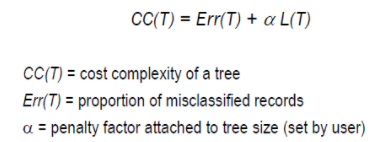
\includegraphics[width=0.4\linewidth]{./Figures/Fig_CC.png}
    \caption{Cost complexity of a tree}
    \label{Fig_CC}
\end{figure}

\begin{table}[H]
\begin{tabular}{p{0.2\textwidth}p{0.2\textwidth}p{0.1\textwidth}p{0.4\textwidth}}
    \toprule
    \textbf{Hyperparameter} & \textbf{Description }  & \textbf{Final Value} & \textbf{Interpretation} \\
    \midrule
    colsample-bytree & Percentage of features used per tree & 0.5 & High values can lead to overfitting\\
    \hline
    learning rate & The learning rate corresponds to how quickly the error is corrected from each tree to the next and is a simple multiplier 0\<LR\≤1 & 0.08 & Chosen to prevent overfitting, usually a value between 0.05 and 0.3 is chosen\\
    \hline
    n-estimators  & Number of trees on which the prediction is calculated based on mean computation & 500 & 500 decision trees are used, which lies in the typical range of 100 to 1.000 trees and should be sufficient for generalizable prediction. The relatively small learning rate requires a certain amount of trees.\\
    \hline
    max_depth & Determines how deeply each tree is allowed to grow during any boosting round & 6 & A tree size of 6 is higher than the default of 3, meaning it  can grow more than default.\\
    \hline
    subsample & Percentage of samples used by tree & 1 & Low values can cause underfitting. The hyperparameter tuning increased the subsample value from 0.8 to 1 \\
     \hline
     gamma & Regularization parameter controlling the splitting of nodes (Minimum loss reduction required to make a further partition on a leaf node of the tree). & 0.6 & The larger gamma is, the more conservative the algorithm will be, that is why 0.6 was chosen\\
 
    \bottomrule
\end{tabular}
\caption{\label{table:isabel}Isabel}
\end{table}








